% Self-contained manuscript: all text, tables, macros, proofs, and references are inline.
% Edit this file; separate section/table sources are retained snapshots, not build inputs.
% External dependencies: figure assets, the ICLR style, and standard LaTeX packages.
% Build: tectonic -X compile main-updated.tex --keep-logs --keep-intermediates
% The original main.tex and refs.bib are preserved.
\documentclass{article}
\usepackage[T1]{fontenc}
\usepackage{iclr2027_conference,times}
% BEGIN inlined content: math_commands.tex
%%%%% NEW MATH DEFINITIONS %%%%%

\usepackage{amsmath,amsfonts,bm}

% Mark sections of captions for referring to divisions of figures
\newcommand{\figleft}{{\em (Left)}}
\newcommand{\figcenter}{{\em (Center)}}
\newcommand{\figright}{{\em (Right)}}
\newcommand{\figtop}{{\em (Top)}}
\newcommand{\figbottom}{{\em (Bottom)}}
\newcommand{\captiona}{{\em (a)}}
\newcommand{\captionb}{{\em (b)}}
\newcommand{\captionc}{{\em (c)}}
\newcommand{\captiond}{{\em (d)}}

% Highlight a newly defined term
\newcommand{\newterm}[1]{{\bf #1}}


% Figure reference, lower-case.
\def\figref#1{figure~\ref{#1}}
% Figure reference, capital. For start of sentence
\def\Figref#1{Figure~\ref{#1}}
\def\twofigref#1#2{figures \ref{#1} and \ref{#2}}
\def\quadfigref#1#2#3#4{figures \ref{#1}, \ref{#2}, \ref{#3} and \ref{#4}}
% Section reference, lower-case.
\def\secref#1{section~\ref{#1}}
% Section reference, capital.
\def\Secref#1{Section~\ref{#1}}
% Reference to two sections.
\def\twosecrefs#1#2{sections \ref{#1} and \ref{#2}}
% Reference to three sections.
\def\secrefs#1#2#3{sections \ref{#1}, \ref{#2} and \ref{#3}}
% Reference to an equation, lower-case.
\def\eqref#1{equation~\ref{#1}}
% Reference to an equation, upper case
\def\Eqref#1{Equation~\ref{#1}}
% A raw reference to an equation---avoid using if possible
\def\plaineqref#1{\ref{#1}}
% Reference to a chapter, lower-case.
\def\chapref#1{chapter~\ref{#1}}
% Reference to an equation, upper case.
\def\Chapref#1{Chapter~\ref{#1}}
% Reference to a range of chapters
\def\rangechapref#1#2{chapters\ref{#1}--\ref{#2}}
% Reference to an algorithm, lower-case.
\def\algref#1{algorithm~\ref{#1}}
% Reference to an algorithm, upper case.
\def\Algref#1{Algorithm~\ref{#1}}
\def\twoalgref#1#2{algorithms \ref{#1} and \ref{#2}}
\def\Twoalgref#1#2{Algorithms \ref{#1} and \ref{#2}}
% Reference to a part, lower case
\def\partref#1{part~\ref{#1}}
% Reference to a part, upper case
\def\Partref#1{Part~\ref{#1}}
\def\twopartref#1#2{parts \ref{#1} and \ref{#2}}

\def\ceil#1{\lceil #1 \rceil}
\def\floor#1{\lfloor #1 \rfloor}
\def\1{\bm{1}}
\newcommand{\train}{\mathcal{D}}
\newcommand{\valid}{\mathcal{D_{\mathrm{valid}}}}
\newcommand{\test}{\mathcal{D_{\mathrm{test}}}}

\def\eps{{\epsilon}}


% Random variables
\def\reta{{\textnormal{$\eta$}}}
\def\ra{{\textnormal{a}}}
\def\rb{{\textnormal{b}}}
\def\rc{{\textnormal{c}}}
\def\rd{{\textnormal{d}}}
\def\re{{\textnormal{e}}}
\def\rf{{\textnormal{f}}}
\def\rg{{\textnormal{g}}}
\def\rh{{\textnormal{h}}}
\def\ri{{\textnormal{i}}}
\def\rj{{\textnormal{j}}}
\def\rk{{\textnormal{k}}}
\def\rl{{\textnormal{l}}}
% rm is already a command, just don't name any random variables m
\def\rn{{\textnormal{n}}}
\def\ro{{\textnormal{o}}}
\def\rp{{\textnormal{p}}}
\def\rq{{\textnormal{q}}}
\def\rr{{\textnormal{r}}}
\def\rs{{\textnormal{s}}}
\def\rt{{\textnormal{t}}}
\def\ru{{\textnormal{u}}}
\def\rv{{\textnormal{v}}}
\def\rw{{\textnormal{w}}}
\def\rx{{\textnormal{x}}}
\def\ry{{\textnormal{y}}}
\def\rz{{\textnormal{z}}}

% Random vectors
\def\rvepsilon{{\mathbf{\epsilon}}}
\def\rvtheta{{\mathbf{\theta}}}
\def\rva{{\mathbf{a}}}
\def\rvb{{\mathbf{b}}}
\def\rvc{{\mathbf{c}}}
\def\rvd{{\mathbf{d}}}
\def\rve{{\mathbf{e}}}
\def\rvf{{\mathbf{f}}}
\def\rvg{{\mathbf{g}}}
\def\rvh{{\mathbf{h}}}
\def\rvu{{\mathbf{i}}}
\def\rvj{{\mathbf{j}}}
\def\rvk{{\mathbf{k}}}
\def\rvl{{\mathbf{l}}}
\def\rvm{{\mathbf{m}}}
\def\rvn{{\mathbf{n}}}
\def\rvo{{\mathbf{o}}}
\def\rvp{{\mathbf{p}}}
\def\rvq{{\mathbf{q}}}
\def\rvr{{\mathbf{r}}}
\def\rvs{{\mathbf{s}}}
\def\rvt{{\mathbf{t}}}
\def\rvu{{\mathbf{u}}}
\def\rvv{{\mathbf{v}}}
\def\rvw{{\mathbf{w}}}
\def\rvx{{\mathbf{x}}}
\def\rvy{{\mathbf{y}}}
\def\rvz{{\mathbf{z}}}

% Elements of random vectors
\def\erva{{\textnormal{a}}}
\def\ervb{{\textnormal{b}}}
\def\ervc{{\textnormal{c}}}
\def\ervd{{\textnormal{d}}}
\def\erve{{\textnormal{e}}}
\def\ervf{{\textnormal{f}}}
\def\ervg{{\textnormal{g}}}
\def\ervh{{\textnormal{h}}}
\def\ervi{{\textnormal{i}}}
\def\ervj{{\textnormal{j}}}
\def\ervk{{\textnormal{k}}}
\def\ervl{{\textnormal{l}}}
\def\ervm{{\textnormal{m}}}
\def\ervn{{\textnormal{n}}}
\def\ervo{{\textnormal{o}}}
\def\ervp{{\textnormal{p}}}
\def\ervq{{\textnormal{q}}}
\def\ervr{{\textnormal{r}}}
\def\ervs{{\textnormal{s}}}
\def\ervt{{\textnormal{t}}}
\def\ervu{{\textnormal{u}}}
\def\ervv{{\textnormal{v}}}
\def\ervw{{\textnormal{w}}}
\def\ervx{{\textnormal{x}}}
\def\ervy{{\textnormal{y}}}
\def\ervz{{\textnormal{z}}}

% Random matrices
\def\rmA{{\mathbf{A}}}
\def\rmB{{\mathbf{B}}}
\def\rmC{{\mathbf{C}}}
\def\rmD{{\mathbf{D}}}
\def\rmE{{\mathbf{E}}}
\def\rmF{{\mathbf{F}}}
\def\rmG{{\mathbf{G}}}
\def\rmH{{\mathbf{H}}}
\def\rmI{{\mathbf{I}}}
\def\rmJ{{\mathbf{J}}}
\def\rmK{{\mathbf{K}}}
\def\rmL{{\mathbf{L}}}
\def\rmM{{\mathbf{M}}}
\def\rmN{{\mathbf{N}}}
\def\rmO{{\mathbf{O}}}
\def\rmP{{\mathbf{P}}}
\def\rmQ{{\mathbf{Q}}}
\def\rmR{{\mathbf{R}}}
\def\rmS{{\mathbf{S}}}
\def\rmT{{\mathbf{T}}}
\def\rmU{{\mathbf{U}}}
\def\rmV{{\mathbf{V}}}
\def\rmW{{\mathbf{W}}}
\def\rmX{{\mathbf{X}}}
\def\rmY{{\mathbf{Y}}}
\def\rmZ{{\mathbf{Z}}}

% Elements of random matrices
\def\ermA{{\textnormal{A}}}
\def\ermB{{\textnormal{B}}}
\def\ermC{{\textnormal{C}}}
\def\ermD{{\textnormal{D}}}
\def\ermE{{\textnormal{E}}}
\def\ermF{{\textnormal{F}}}
\def\ermG{{\textnormal{G}}}
\def\ermH{{\textnormal{H}}}
\def\ermI{{\textnormal{I}}}
\def\ermJ{{\textnormal{J}}}
\def\ermK{{\textnormal{K}}}
\def\ermL{{\textnormal{L}}}
\def\ermM{{\textnormal{M}}}
\def\ermN{{\textnormal{N}}}
\def\ermO{{\textnormal{O}}}
\def\ermP{{\textnormal{P}}}
\def\ermQ{{\textnormal{Q}}}
\def\ermR{{\textnormal{R}}}
\def\ermS{{\textnormal{S}}}
\def\ermT{{\textnormal{T}}}
\def\ermU{{\textnormal{U}}}
\def\ermV{{\textnormal{V}}}
\def\ermW{{\textnormal{W}}}
\def\ermX{{\textnormal{X}}}
\def\ermY{{\textnormal{Y}}}
\def\ermZ{{\textnormal{Z}}}

% Vectors
\def\vzero{{\bm{0}}}
\def\vone{{\bm{1}}}
\def\vmu{{\bm{\mu}}}
\def\vtheta{{\bm{\theta}}}
\def\va{{\bm{a}}}
\def\vb{{\bm{b}}}
\def\vc{{\bm{c}}}
\def\vd{{\bm{d}}}
\def\ve{{\bm{e}}}
\def\vf{{\bm{f}}}
\def\vg{{\bm{g}}}
\def\vh{{\bm{h}}}
\def\vi{{\bm{i}}}
\def\vj{{\bm{j}}}
\def\vk{{\bm{k}}}
\def\vl{{\bm{l}}}
\def\vm{{\bm{m}}}
\def\vn{{\bm{n}}}
\def\vo{{\bm{o}}}
\def\vp{{\bm{p}}}
\def\vq{{\bm{q}}}
\def\vr{{\bm{r}}}
\def\vs{{\bm{s}}}
\def\vt{{\bm{t}}}
\def\vu{{\bm{u}}}
\def\vv{{\bm{v}}}
\def\vw{{\bm{w}}}
\def\vx{{\bm{x}}}
\def\vy{{\bm{y}}}
\def\vz{{\bm{z}}}

% Elements of vectors
\def\evalpha{{\alpha}}
\def\evbeta{{\beta}}
\def\evepsilon{{\epsilon}}
\def\evlambda{{\lambda}}
\def\evomega{{\omega}}
\def\evmu{{\mu}}
\def\evpsi{{\psi}}
\def\evsigma{{\sigma}}
\def\evtheta{{\theta}}
\def\eva{{a}}
\def\evb{{b}}
\def\evc{{c}}
\def\evd{{d}}
\def\eve{{e}}
\def\evf{{f}}
\def\evg{{g}}
\def\evh{{h}}
\def\evi{{i}}
\def\evj{{j}}
\def\evk{{k}}
\def\evl{{l}}
\def\evm{{m}}
\def\evn{{n}}
\def\evo{{o}}
\def\evp{{p}}
\def\evq{{q}}
\def\evr{{r}}
\def\evs{{s}}
\def\evt{{t}}
\def\evu{{u}}
\def\evv{{v}}
\def\evw{{w}}
\def\evx{{x}}
\def\evy{{y}}
\def\evz{{z}}

% Matrix
\def\mA{{\bm{A}}}
\def\mB{{\bm{B}}}
\def\mC{{\bm{C}}}
\def\mD{{\bm{D}}}
\def\mE{{\bm{E}}}
\def\mF{{\bm{F}}}
\def\mG{{\bm{G}}}
\def\mH{{\bm{H}}}
\def\mI{{\bm{I}}}
\def\mJ{{\bm{J}}}
\def\mK{{\bm{K}}}
\def\mL{{\bm{L}}}
\def\mM{{\bm{M}}}
\def\mN{{\bm{N}}}
\def\mO{{\bm{O}}}
\def\mP{{\bm{P}}}
\def\mQ{{\bm{Q}}}
\def\mR{{\bm{R}}}
\def\mS{{\bm{S}}}
\def\mT{{\bm{T}}}
\def\mU{{\bm{U}}}
\def\mV{{\bm{V}}}
\def\mW{{\bm{W}}}
\def\mX{{\bm{X}}}
\def\mY{{\bm{Y}}}
\def\mZ{{\bm{Z}}}
\def\mBeta{{\bm{\beta}}}
\def\mPhi{{\bm{\Phi}}}
\def\mLambda{{\bm{\Lambda}}}
\def\mSigma{{\bm{\Sigma}}}

% Tensor
\DeclareMathAlphabet{\mathsfit}{\encodingdefault}{\sfdefault}{m}{sl}
\SetMathAlphabet{\mathsfit}{bold}{\encodingdefault}{\sfdefault}{bx}{n}
\newcommand{\tens}[1]{\bm{\mathsfit{#1}}}
\def\tA{{\tens{A}}}
\def\tB{{\tens{B}}}
\def\tC{{\tens{C}}}
\def\tD{{\tens{D}}}
\def\tE{{\tens{E}}}
\def\tF{{\tens{F}}}
\def\tG{{\tens{G}}}
\def\tH{{\tens{H}}}
\def\tI{{\tens{I}}}
\def\tJ{{\tens{J}}}
\def\tK{{\tens{K}}}
\def\tL{{\tens{L}}}
\def\tM{{\tens{M}}}
\def\tN{{\tens{N}}}
\def\tO{{\tens{O}}}
\def\tP{{\tens{P}}}
\def\tQ{{\tens{Q}}}
\def\tR{{\tens{R}}}
\def\tS{{\tens{S}}}
\def\tT{{\tens{T}}}
\def\tU{{\tens{U}}}
\def\tV{{\tens{V}}}
\def\tW{{\tens{W}}}
\def\tX{{\tens{X}}}
\def\tY{{\tens{Y}}}
\def\tZ{{\tens{Z}}}


% Graph
\def\gA{{\mathcal{A}}}
\def\gB{{\mathcal{B}}}
\def\gC{{\mathcal{C}}}
\def\gD{{\mathcal{D}}}
\def\gE{{\mathcal{E}}}
\def\gF{{\mathcal{F}}}
\def\gG{{\mathcal{G}}}
\def\gH{{\mathcal{H}}}
\def\gI{{\mathcal{I}}}
\def\gJ{{\mathcal{J}}}
\def\gK{{\mathcal{K}}}
\def\gL{{\mathcal{L}}}
\def\gM{{\mathcal{M}}}
\def\gN{{\mathcal{N}}}
\def\gO{{\mathcal{O}}}
\def\gP{{\mathcal{P}}}
\def\gQ{{\mathcal{Q}}}
\def\gR{{\mathcal{R}}}
\def\gS{{\mathcal{S}}}
\def\gT{{\mathcal{T}}}
\def\gU{{\mathcal{U}}}
\def\gV{{\mathcal{V}}}
\def\gW{{\mathcal{W}}}
\def\gX{{\mathcal{X}}}
\def\gY{{\mathcal{Y}}}
\def\gZ{{\mathcal{Z}}}

% Sets
\def\sA{{\mathbb{A}}}
\def\sB{{\mathbb{B}}}
\def\sC{{\mathbb{C}}}
\def\sD{{\mathbb{D}}}
% Don't use a set called E, because this would be the same as our symbol
% for expectation.
\def\sF{{\mathbb{F}}}
\def\sG{{\mathbb{G}}}
\def\sH{{\mathbb{H}}}
\def\sI{{\mathbb{I}}}
\def\sJ{{\mathbb{J}}}
\def\sK{{\mathbb{K}}}
\def\sL{{\mathbb{L}}}
\def\sM{{\mathbb{M}}}
\def\sN{{\mathbb{N}}}
\def\sO{{\mathbb{O}}}
\def\sP{{\mathbb{P}}}
\def\sQ{{\mathbb{Q}}}
\def\sR{{\mathbb{R}}}
\def\sS{{\mathbb{S}}}
\def\sT{{\mathbb{T}}}
\def\sU{{\mathbb{U}}}
\def\sV{{\mathbb{V}}}
\def\sW{{\mathbb{W}}}
\def\sX{{\mathbb{X}}}
\def\sY{{\mathbb{Y}}}
\def\sZ{{\mathbb{Z}}}

% Entries of a matrix
\def\emLambda{{\Lambda}}
\def\emA{{A}}
\def\emB{{B}}
\def\emC{{C}}
\def\emD{{D}}
\def\emE{{E}}
\def\emF{{F}}
\def\emG{{G}}
\def\emH{{H}}
\def\emI{{I}}
\def\emJ{{J}}
\def\emK{{K}}
\def\emL{{L}}
\def\emM{{M}}
\def\emN{{N}}
\def\emO{{O}}
\def\emP{{P}}
\def\emQ{{Q}}
\def\emR{{R}}
\def\emS{{S}}
\def\emT{{T}}
\def\emU{{U}}
\def\emV{{V}}
\def\emW{{W}}
\def\emX{{X}}
\def\emY{{Y}}
\def\emZ{{Z}}
\def\emSigma{{\Sigma}}

% entries of a tensor
% Same font as tensor, without \bm wrapper
\newcommand{\etens}[1]{\mathsfit{#1}}
\def\etLambda{{\etens{\Lambda}}}
\def\etA{{\etens{A}}}
\def\etB{{\etens{B}}}
\def\etC{{\etens{C}}}
\def\etD{{\etens{D}}}
\def\etE{{\etens{E}}}
\def\etF{{\etens{F}}}
\def\etG{{\etens{G}}}
\def\etH{{\etens{H}}}
\def\etI{{\etens{I}}}
\def\etJ{{\etens{J}}}
\def\etK{{\etens{K}}}
\def\etL{{\etens{L}}}
\def\etM{{\etens{M}}}
\def\etN{{\etens{N}}}
\def\etO{{\etens{O}}}
\def\etP{{\etens{P}}}
\def\etQ{{\etens{Q}}}
\def\etR{{\etens{R}}}
\def\etS{{\etens{S}}}
\def\etT{{\etens{T}}}
\def\etU{{\etens{U}}}
\def\etV{{\etens{V}}}
\def\etW{{\etens{W}}}
\def\etX{{\etens{X}}}
\def\etY{{\etens{Y}}}
\def\etZ{{\etens{Z}}}

% The true underlying data generating distribution
\newcommand{\pdata}{p_{\rm{data}}}
% The empirical distribution defined by the training set
\newcommand{\ptrain}{\hat{p}_{\rm{data}}}
\newcommand{\Ptrain}{\hat{P}_{\rm{data}}}
% The model distribution
\newcommand{\pmodel}{p_{\rm{model}}}
\newcommand{\Pmodel}{P_{\rm{model}}}
\newcommand{\ptildemodel}{\tilde{p}_{\rm{model}}}
% Stochastic autoencoder distributions
\newcommand{\pencode}{p_{\rm{encoder}}}
\newcommand{\pdecode}{p_{\rm{decoder}}}
\newcommand{\precons}{p_{\rm{reconstruct}}}

\newcommand{\laplace}{\mathrm{Laplace}} % Laplace distribution

\newcommand{\E}{\mathbb{E}}
\newcommand{\Ls}{\mathcal{L}}
\newcommand{\R}{\mathbb{R}}
\newcommand{\emp}{\tilde{p}}
\newcommand{\lr}{\alpha}
\newcommand{\reg}{\lambda}
\newcommand{\rect}{\mathrm{rectifier}}
\newcommand{\softmax}{\mathrm{softmax}}
\newcommand{\sigmoid}{\sigma}
\newcommand{\softplus}{\zeta}
\newcommand{\KL}{D_{\mathrm{KL}}}
\newcommand{\Var}{\mathrm{Var}}
\newcommand{\standarderror}{\mathrm{SE}}
\newcommand{\Cov}{\mathrm{Cov}}
% Wolfram Mathworld says $L^2$ is for function spaces and $\ell^2$ is for vectors
% But then they seem to use $L^2$ for vectors throughout the site, and so does
% wikipedia.
\newcommand{\normlzero}{L^0}
\newcommand{\normlone}{L^1}
\newcommand{\normltwo}{L^2}
\newcommand{\normlp}{L^p}
\newcommand{\normmax}{L^\infty}

\newcommand{\parents}{Pa} % See usage in notation.tex. Chosen to match Daphne's book.

\DeclareMathOperator*{\argmax}{arg\,max}
\DeclareMathOperator*{\argmin}{arg\,min}

\DeclareMathOperator{\sign}{sign}
\DeclareMathOperator{\Tr}{Tr}
\let\ab\allowbreak
% END inlined content: math_commands.tex
\usepackage{amssymb,amsthm}
\usepackage{booktabs,array,multirow,tabularx}
\usepackage{graphicx,xcolor,enumitem,capt-of}
\usepackage{algorithm,algorithmic}
\usepackage{hyperref}
\usepackage{url}
\usepackage[nameinlink,noabbrev]{cleveref}
\graphicspath{{figures/}}
\newcommand{\z}{z}
\newcommand{\psiT}{\psi}
\newcommand{\Htd}{r_{\mathrm{TD}}}
\newcommand{\ET}{\mathrm{ET}}
\newcommand{\dd}{d_{\psi}}
\newcommand{\ind}{\mathbf{1}}
\newcommand{\Rset}{\mathcal R_\lambda}
\newcommand{\EE}{\mathbb E}
\newcommand{\PP}{\mathbb P}
\newcommand{\Aset}{\mathcal A}
\newcommand{\pos}[1]{[#1]_+}
\newtheorem{theorem}{Theorem}
\newtheorem{lemma}[theorem]{Lemma}
\newtheorem{proposition}[theorem]{Proposition}
\newtheorem{corollary}[theorem]{Corollary}
\theoremstyle{definition}
\newtheorem{assumption}[theorem]{Assumption}
\newtheorem{definition}[theorem]{Definition}
\theoremstyle{remark}
\newtheorem{remark}[theorem]{Remark}
\crefname{assumption}{Assumption}{Assumptions}
\crefname{proposition}{Proposition}{Propositions}
\crefname{corollary}{Corollary}{Corollaries}
\crefname{lemma}{Lemma}{Lemmas}
\crefname{theorem}{Theorem}{Theorems}
\title{Graph-Guided Long-Horizon MPC with World Models}
\author{Anonymous authors}
% Keep the submission anonymous.
\begin{document}
\maketitle
\begin{abstract}
Terminal latent distance can poorly reflect progress in long-horizon world-model
planning. We add a temporal distance representation, a graph of offline experience,
and a budget-conditioned reachability critic to a frozen LeWorldModel (LeWM).
Graph search supplies an intermediate target. The critic scores predicted endpoints
by the expected time to reach goal, and the controller switches to latent L2 near the goal.
We keep the encoder, predictor, and cross-entropy method (CEM) search settings fixed.
We bound the number of replanning calls needed to reach the goal under explicit
execution, model, search, and critic error conditions. We also bound critic error
across horizons and state when its score equals a truncated expected time to reach the goal.
On fixed evaluation tasks, cross-episode success increases from 14.4 to 42.4\% on Push-T,
29.2 to 65.6\% on Reacher, and 16.4 to 27.6\% on Cube. Improvements are largest beyond one
planning horizon; short-range losses remain on Push-T and Reacher. Ablations show that
graph guidance and the critic are complementary on Push-T, whereas Cube benefits primarily
from the learned temporal representation.
\end{abstract}

\section{Introduction}
Joint-embedding world models enable control by predicting the consequences of candidate
actions in a learned latent space \citep{dinowm,lewm}. Their planning objective often compares a
predicted terminal latent with an encoded goal image. This avoids learning a task-specific
reward, but latent Euclidean distance need not reflect the time or actions required to reach
the goal. On our Push-T tasks, LeWM's terminal-L2 planner succeeds at 91.2\% for goals 25 steps
ahead, 40.8\% at 50 steps, and 13.2\% at 100 steps. Cross-episode success is 14.4\%, despite
replanning every 25 steps.

We use a graph of offline observations to choose intermediate targets.
A temporal distance representation (TDR) organizes frozen latents into a graph.
Graph search selects a cluster along a shortest route to the goal using a calibrated
lookahead distance. CEM then optimizes a combination of distance to that cluster and a
budget-conditioned reachability score. Once the current state is close to the goal in
TDR space, the base cost switches to LeWM's latent L2. The critic remains active.
We train the TDR and critic while keeping the dynamics model fixed; CEM supplies the actions.

Graph connectivity does not ensure executable routes: proximity edges may be infeasible,
and CEM can miss useful actions. We analyze the normalized subgoal and critic cost and prove
finite-time progress and local convergence under explicit execution, model, search,
and observability conditions. We also explain why optimizing reachability separately
at each horizon need not describe the time to reach the goal under any single policy.

The same configuration improves over LeWM at offsets 50 and 100 and on cross-episode
goals in all three environments. On Cube, however, TDR alone achieves higher cross-episode
success than the full method.
Our main contributions are:
\begin{enumerate}[nosep,leftmargin=*]
 \item A graph-guided objective for latent model predictive control (MPC), combining dataset
       subgoals, a remaining-time budget, and a local L2 switch (\cref{sec:method}).
 \item A method-specific progress and convergence analysis, including the effect of CEM
       approximation and population normalization (\cref{sec:theory}).
 \item A controlled comparison on three environments, with component ablations and diagnostics
       that distinguish long-range guidance from local execution (\cref{sec:experiments}).
\end{enumerate}

\section{Related work}
\label{sec:related}
\paragraph{Costs and hierarchies for latent planning.}
LeWM and DINO-WM use predictive latent models for visual planning \citep{lewm,dinowm}.
TRM learns a temporal pairwise cost on a fixed representation \citep{trm};
RC-aux adds reachability supervision during world-model training \citep{rcaux}.
SAGE uses learned subgoals and action proposals, while Hi-LeWM studies how high-level
search interacts with a frozen low-level model \citep{sage,hilewm}.
We choose targets from clusters of dataset observations and keep CEM's action
initialization unchanged in the main configuration.

\paragraph{Graph planning and temporal representations.}
SPTM, SoRB, and SGM combine stored experience with learned local controllers
\citep{sptm,sorb,sgm}. GAS uses a temporal graph to guide a learned policy \citep{gas};
SSE addresses subgoal feasibility through replay of execution outcomes \citep{sse}.
We adapt GAS's graph construction to frozen-model MPC.
PcLast and ALPS already combine cluster-based planning and CEM; ALPS also learns a
behavior prior \citep{pclast,alps}. Our contribution combines a frozen pixel world model,
a survival cost that uses the remaining budget, and a local switch. We prove a
progress bound for their joint objective.
HILP proves goal-reaching results under representation and directional-control errors
\citep{hilp}; quasimetric learning treats the asymmetry of temporal distance explicitly
\citep{qrl}. We analyze how the controller attaches to the graph, executes each full plan,
and normalizes the combined cost.

\paragraph{Values and convergence in MPC.}
POLO and TD-MPC use learned terminal values to complement short model rollouts
\citep{polo,tdmpc,tdmpc2}. Classical MPC stability depends on suitable terminal-region
and local-control conditions \citep{mayne2000}; stochastic shortest-path theory similarly
requires conditions ensuring eventual goal arrival \citep{bertsekas1991}.
Our guarantees likewise require explicit control and goal-reaching assumptions.
We bound graph progress and error propagation; the neural training loss alone does not establish convergence.

\section{Method}
\label{sec:method}
\Cref{fig:approach} summarizes the offline preparation and online planning procedure.
\begin{figure}[t]
 \centering
 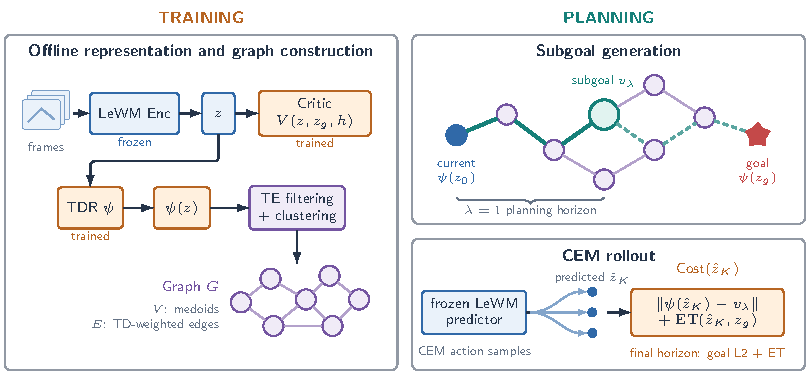
\includegraphics[width=\linewidth]{approach}
 \caption{Graph-guided latent MPC. Offline, the frozen encoder supplies latents for the TDR,
 graph, and reachability critic; critic labels are derived from the TDR, so no stage reads simulator state.
 Online, graph search chooses a target and the frozen predictor rolls out CEM candidates.
 CEM ranks endpoints by combining target distance and the survival score after normalizing
 each over its candidate population. The controller switches the base cost to goal L2
 near the goal. In the schematic,
 $v_\lambda$ denotes the subgoal coordinate $y_q$; edge weights use TDR distance.}
 \label{fig:approach}
\end{figure}

\paragraph{Frozen model and time units.}
The encoder $E$ maps a $224\times224$ image to a 192-dimensional latent.
The LeWM predictor $P$ uses a three-block history.
One action block contains $\Delta=5$ environment actions; CEM plans $K=5$ blocks.
The controller executes $L=K\Delta=25$ steps before replanning, unless it reaches the goal first.
Every main comparison uses 300 candidates, 30 iterations, and 30 elites.
LeWM's base cost is $c_{\mathrm{L2}}(\hat z_K)=\|\hat z_K-z_g\|^2$.
We change the scoring function while retaining the encoder, predictor, and search settings.
All distances without a squared norm below are unsquared Euclidean distances.

\subsection{Temporal representation and graph}
\label{sec:graph}
Write $\dd(z,z')=\|\psi(z)-\psi(z')\|$, with $\psi:\mathbb R^{192}\to\mathbb R^{32}$.
Following HILP and GAS \citep{hilp,gas}, two networks learn the negative-distance value
$U(z,z_g)=-\dd(z,z_g)$ using expectile TD. For a nonterminal transition, the target is
$q=-1+\gamma\min_{i=1,2}U_i^-(z',z_g)$, with $\gamma=0.99$ and EMA targets:
\begin{equation}
 \mathcal L_{\mathrm{TDR}}
 =\EE[\ell_{0.99}(q-U(z,z_g))],
 \qquad \ell_\tau(u)=|\tau-\ind_{\{u<0\}}|u^2.
 \label{eq:tdr}
\end{equation}
We set the goal's terminal value to zero. With probability 0.625, we sample a future
goal frame at a geometric offset with parameter $1-\gamma$; otherwise, we sample
uniformly from the dataset. The learned distance approximates discounted temporal
structure symmetrically. We calibrate its scale using $u_k=\operatorname{median}_t\dd(z_t,z_{t+k})$
on training trajectories.

Graph construction uses radius $\Htd=u_{12}$ in TDR units and a separate integer temporal lag
$k_{\mathrm{TE}}$ in environment steps. Let $F_t$ be the first later frame in the
same episode at TDR distance at least $\Htd$, or the last frame if no such crossing exists.
The temporal-efficiency filter retains frames whose nonzero displacement vectors satisfy
\begin{equation}
 \mathrm{TE}(z_t)=
 \frac{\langle\psi(F_t)-\psi(z_t),\,\psi(z_{t+k_{\mathrm{TE}}})-\psi(z_t)\rangle}
 {\|\psi(F_t)-\psi(z_t)\|\,\|\psi(z_{t+k_{\mathrm{TE}}})-\psi(z_t)\|}
 \ge 0.9 .
 \label{eq:te}
\end{equation}
We clip the lag at the episode end and exclude comparisons with zero displacement.
We cluster retained embeddings sequentially, admitting points within $\Htd/2$ of a center
and updating centers to member means. Node $v$ stores a TDR center $y_v\in\mathbb R^{32}$
and a medoid latent $z_v\in\mathbb R^{192}$.
We link centers at distance at most $\Htd$ with weight $\|y_v-y_w\|$.
These links suggest local connections but do not ensure that the dynamics can execute them.

For a goal, a temporary node at $\psi(z_g)$ connects to centers within
$r_g=\max(\Htd,1.2d_{\min})$, where $d_{\min}=\min_v\|\psi(z_g)-y_v\|$.
Dijkstra's algorithm computes $D_g[v]$, the shortest-path length to this node.
The resulting graphs have approximately 20.5k, 535, and 16k nodes on Push-T, Reacher,
and Cube, respectively. We keep the graph and its distances fixed during each episode.

\subsection{Horizon-matched subgoal and local switch}
\label{sec:subgoal}
At a planning call, restrict attachment to
$A(z_0)=\{v:\|\psi(z_0)-y_v\|\le\Htd,\ D_g[v]<\infty\}$ and choose
\begin{equation}
 v^\star\in\arg\min_{v\in A(z_0)}
       \{\|\psi(z_0)-y_v\|+D_g[v]\}.
 \label{eq:startnode}
\end{equation}
Starting with this attachment segment, follow a shortest path and select the first node
whose cumulative path length reaches $\lambda=u_{25}$, or the goal if the path ends earlier.
Denote its coordinate by $y_q$. Selecting the first crossing can overshoot $\lambda$
by one edge. The theory assumes that an action sequence can reach near this target;
median calibration alone does not establish that assumption.
The base cost is
\begin{equation}
 b(\hat z_K)=
 \begin{cases}
   \|\hat z_K-z_g\|^2,& \dd(z_0,z_g)\le\lambda,\\
   \|\psi(\hat z_K)-y_q\|,& \dd(z_0,z_g)>\lambda .
 \end{cases}
 \label{eq:subgoal}
\end{equation}
The controller recomputes the switching decision at each call.
The graph branch requires $A(z_0)\ne\varnothing$; disconnected or unattached states
have no finite route to follow. The controller uses the nearest node as a fallback in this case,
but the graph-progress theorem does not cover that fallback.

\subsection{Reachability score and the remaining budget}
\label{sec:critic}
We query the five-member critic ensemble $V(z,z_g,h)\in[0,1]$ at
$h=0,5,\ldots,50$. We train it with binary cross-entropy on hindsight first-hit labels
$\ind_{\{\tau\le h\}}$, cross-episode negatives, and predicted latents under logged
actions. Here $\tau$ is the first logged step with $\dd(z_{t+k},z_g)<u_2$.
Cross-episode pairs receive label $0$ only when $\dd(z,z_g)\ge 1.25\,u_{\max(h,5)}$,
that is, when the TDR places the goal beyond budget $h$.
No label reads the simulator state, so training and inference are both pixel-only;
on Push-T, the TDR-derived $\tau$ agrees with the success predicate on 97.7\% of draws.
For $h\ge\Delta$ at unsuccessful states, we sample $M$ blocks around the logged action and use
\begin{equation}
 q_h=\max_{m\le M}
 \operatorname{clip}_{[0,1]}
 \{\bar V(\hat z'_m,z_g,h-\Delta)-\kappa\bar\sigma(\hat z'_m,z_g,h-\Delta)\},
 \quad \kappa=1 .
 \label{eq:critic-bootstrap}
\end{equation}
A hinge loss penalizes $[V(z,z_g,h)-V(z,z_g,h+\Delta)]_+$.
Here $\bar V,\bar\sigma$ are the EMA ensemble mean and standard deviation.
The TDR-derived labels and the ensemble penalty are heuristics:
a TDR ball is only a proxy for the goal condition, a TDR distance threshold is not a
physical reachability bound,
and ensemble spread is not a calibrated confidence interval.
We therefore treat the critic as an approximate reachability score and account for its
error relative to a specified control process in \cref{sec:theory}.

Let $B$ be the budget and $t$ the executed steps. For a full plan with $B-t\ge L$,
set $h_{\mathrm{rem}}=\min(50,B-t-L)$ and
$n=\lfloor h_{\mathrm{rem}}/\Delta\rfloor$. We sum over all grid points, including both endpoints:
\begin{equation}
 \ET(\hat z_K,z_g)=\Delta\sum_{j=0}^{n}
                    [1-V(\hat z_K,z_g,j\Delta)],\qquad C_n=(n+1)\Delta.
 \label{eq:et}
\end{equation}
The cap is $C_n$, one grid interval beyond the largest queried deadline.
When no time remains, the score still penalizes predicted failure at the endpoint.
The score equals a truncated expected \emph{grid} hitting time only when all queried
probabilities describe the same continuation policy. Otherwise, we use it as a sum of
reachability estimates. Updating the budget prevents queries beyond the available time;
it does not guarantee success by the deadline.

At each CEM iteration, we normalize each cost over the candidate population using
$\widetilde f=(f-\operatorname{median}f)/s_f$, where
$s_f=\max(\operatorname{IQR}f,\nu_f)$. The fixed positive floor $\nu_f$ prevents division by zero.
The objective is
\begin{equation}
 c=\widetilde b+\beta\widetilde{\ET},\qquad \beta=1.
 \label{eq:compose}
\end{equation}
Although $\beta$ is fixed, the effective relative weight in unnormalized units is
$\beta s_b/s_{\ET}$. This ratio is central to the progress bound.
The TDR and critic train for 50k and 60k updates; \cref{app:hyperparams,app:algorithm}
give the remaining settings and planning pseudocode.

% BEGIN inlined content: theory-main.tex
\section{Theory: from the planning cost to goal progress}
\label{sec:theory}
We analyze the normalized graph and critic cost with the trained networks and graph
held fixed. Our main result bounds graph progress and local convergence without
assuming a globally accurate temporal metric. \Cref{app:theory} connects each assumption
to the algorithm and provides the proofs.
Fix a goal $g$. Define the remaining graph distance $\Phi$ by the attachment objective,
\begin{equation}
 \Phi(z)=\min_{v\in A(z)}\{\|\psi(z)-y_v\|+D_g[v]\},
 \qquad \Rset=\{z:\dd(z,z_g)\le\lambda\}.
 \label{eq:potential}
\end{equation}
For deterministic execution, we analyze CEM's returned sequence using the predictor's input history.
The controller ends the episode as soon as the agent satisfies the environment's goal condition.
\Cref{app:stochastic} covers stochastic execution.

\begin{theorem}[Normalized-cost graph progress]
\label{thm:graph-progress}
Suppose $z\notin\Rset$ has a finite attachment, and let $y_q$ be the first
$\lambda$-crossing target on its selected path.
Write $z^+(u),\hat z^+(u)$ for the true and predicted endpoints of an $L$-step sequence.
Suppose a feasible comparison sequence $u^\circ$ satisfies
$\|\psi(z^+(u^\circ))-y_q\|\le\eta$.
For both $u^\circ$ and the executed sequence $\hat u$, assume
$\|\psi(\hat z^+(u))-\psi(z^+(u))\|\le e_\psi$.
Use the final population's positive scales $s_b,s_S$ and medians for both costs, and suppose
$\hat c(\hat u)\le\hat c(u^\circ)+\epsilon_{\mathrm{opt}}$.
If
$[\widehat S(u^\circ)-\widehat S(\hat u)]_+\le\omega$ for the ET scores, define
\begin{equation}
 \rho=\eta+2e_\psi+s_b\epsilon_{\mathrm{opt}}
                  +\beta\frac{s_b}{s_S}\omega .
 \label{eq:rho}
\end{equation}
If $\rho\le\Htd$ and $\rho<\lambda$, the controller either reaches the goal during the call,
enters $\Rset$, or reduces the remaining graph distance:
\begin{equation}
 \Phi(z^+(\hat u))\le\Phi(z)-(\lambda-\rho).
 \label{eq:graph-descent}
\end{equation}
If these bounds hold at every graph call before stopping, success or entry into $\Rset$ occurs within
$N_G=\lceil\Phi(z_0)/(\lambda-\rho)\rceil$ calls.
\end{theorem}

An endpoint within $\Htd$ of a regular target node can attach there for the next call,
reducing the remaining graph distance by at least $\lambda-\rho$.
If the target is the goal node, the endpoint enters the local region instead.
The bound includes the normalization ratio in \cref{eq:rho}; $\omega=C_n$ always bounds
the critic difference but may be too large to prove progress. Median calibration alone
does not ensure that the comparison sequence exists. \Cref{prop:critic-screen} also
shows when the critic rejects poor plans that subgoal distance alone would favor.

\begin{theorem}[Local convergence after the switch]
\label{thm:local}
Assume the switched controller stays in $\Rset$ until success and enters with
$e(z)=\|z-z_g\|\le R$. Assume $e(z)\le r_{\mathrm{goal}}$ implies the environment's
goal condition. At each local call, suppose a feasible comparison sequence reduces true
latent error to at most $a e(z)$, where $0<a<1$.
Suppose endpoint prediction error is at most $e_z$ for the comparison and executed
sequences, and the normalized solver and critic bounds of \cref{thm:graph-progress}
hold with local constants. Put
\begin{equation}
 d_\ell=2e_z+
 \sqrt{s_b\epsilon_{\mathrm{opt}}+\beta(s_b/s_S)\omega_\ell},
 \qquad e_\infty=\frac{d_\ell}{1-a}.
 \label{eq:local-floor}
\end{equation}
Until success, $e(z_m)\le a^mR+(1-a^m)e_\infty$.
If $e_\infty<r_{\mathrm{goal}}$, success follows within
\[
 N_\ell=\max\!\left\{0,\left\lceil
 \frac{\log(R/(r_{\mathrm{goal}}-e_\infty))}{\log(1/a)}
 \right\rceil\right\}
\]
local calls, with $N_\ell=0$ if $R=0$.
Together with \cref{thm:graph-progress}, $L(N_G+N_\ell)$ is a sufficient execution budget,
provided the bounds hold for every remaining-budget value encountered.
\end{theorem}

These assumptions require the local controller to stay in the switching region and
reduce latent error enough to satisfy the task's goal condition. They play the same role
as local control and terminal-region conditions in MPC \citep{mayne2000}.
The reported success rates alone do not establish them.

\begin{theorem}[Finite-horizon critic error propagation]
\label{thm:critic}
Use a Markov state sufficient to specify block-transition probabilities and the goal condition. After success,
keep the process in a successful state. Let $V_j^*$ be the optimal probability of reaching the goal by $j$
blocks: $V_0^*=\ind_g$ and $V_j^*=\mathcal B V_{j-1}^*$, where $\mathcal B$ is the
undiscounted reachability Bellman operator.
For estimates $\hat V_j$, suppose
$\|\hat V_0-V_0^*\|_\infty\le\varepsilon_0$ and
$\|\hat V_j-\mathcal B\hat V_{j-1}\|_\infty\le\xi_j$.
Then
\begin{align}
 \|\hat V_j-V_j^*\|_\infty
 &\le\varepsilon_0+\sum_{i=1}^j\xi_i, \notag\\
 \left|\Delta\sum_{j=0}^n(1-\hat V_j)
       -\Delta\sum_{j=0}^n(1-V_j^*)\right|
 &\le\Delta\!\left[(n+1)\varepsilon_0+
                      \sum_{i=1}^n(n-i+1)\xi_i\right].
 \label{eq:critic-bound}
\end{align}
Exact synchronous backups with the boundary held fixed recover horizons through $n$
after $n$ sweeps, from any bounded initialization of the other horizons.
\end{theorem}

We apply standard reachability dynamic programming \citep{abate2008} to this critic.
Its residuals include model, action-search, label, and fitting errors; the training loss
alone does not bound them. For a common continuation policy $\pi$, the sum of survival
probabilities is exactly $\EE_\pi\min(T^\pi,C_n)$ for grid hitting time $T^\pi$.
For horizon-wise optimal values it is only a lower bound on
$\inf_\pi\EE_\pi\min(T^\pi,C_n)$ (\cref{prop:policy-consistency}).
Thus ET need not describe any single policy or guarantee success by the deadline.
\Cref{app:expectile} proves the separate tabular expectile convergence result and explains
why it does not imply neural TDR convergence.

\paragraph{Why improvement over terminal L2 is possible.}
\Cref{prop:l2-separation} constructs a problem with an exact model and latents on a circle.
A $K$-block L2 planner stays at the start forever, while the graph objective with an exact
critic reaches the goal in two calls, including $K=5$. Reaching the goal requires a temporary
increase in L2 distance, which the short-horizon L2 planner avoids. This example explains
one advantage; incorrect edges, poor action coverage, or a conflicting critic can reverse it.
% END inlined content: theory-main.tex

\section{Experiments}
\label{sec:experiments}
\subsection{Setup}
\label{sec:setup}
\paragraph{Environments and protocols.}
We use the public LeWM datasets and checkpoints: 18,685 Push-T expert episodes
(2.34M frames), and 10,000 episodes of 201 frames each for Reacher and OGBench Cube
\citep{lewm,ogbench}. Push-T success requires agent and block position errors below
20\,px and block angle error below $\pi/9$. Reacher uses raw joint-angle differences
below 0.05\,rad for both joints, without angle wrapping. Cube requires cube-position
error below 0.04\,m, without an orientation or end-effector condition.
The Reacher convention distinguishes unwrapped joint coordinates and therefore need not
be identifiable from a single image.

Same-episode goals are $H\in\{25,50,100\}$ environment steps after the start,
with budget $B=2H$. Cross-episode tasks draw frames from different episodes, reject
pairs already successful at the start, and impose no additional distance or reachability
filter. Their budgets are 250 steps on Push-T and 200 on Reacher and Cube.
Each protocol uses the same 50 evaluation tasks across methods and five seeds.
For our planner, seeds vary TDR, graph, critic, and CEM randomness; L2 seeds vary
CEM alone. Standard deviations measure variation across seeds on these fixed tasks.
They do not measure uncertainty across new tasks or establish generalization to unseen goals.

\paragraph{Baselines.}
L2 uses LeWM's terminal cost. TDR uses $\dd(\hat z_K,z_g)$ directly.
The graph cost-to-go (CTG) baseline uses a terminal attachment cost plus $D_g$ without
committing to a subgoal. Random samples environment actions uniformly.
We train GCIQL on frozen LeWM latents with the released configuration,
ten epochs per phase, and one training seed on Push-T.
All planning comparisons use the same main CEM configuration.
Panel (B) of \cref{tab:main} gives published results for context.
Those evaluations use different tasks from our matched comparison (\cref{app:published}).

% BEGIN inlined content: tables-main.tex
\begin{table}[t]
\centering\small
\caption{Success (\%). \textbf{(A)} Mean $\pm$ seed standard deviation on 50 fixed tasks and five seeds. Bold marks the best mean. Underlining marks overlap with the best method's mean $\pm$ standard deviation; it does not indicate statistical significance. $^\dagger$GCIQL uses one training seed and a deterministic policy. \textbf{(B)} \citet{lewm}'s published results and our offset-25 means use different tasks, so this panel provides context rather than a matched comparison. ``--'': not reported.}
\label{tab:main}
\textbf{(A) Our results}\par\smallskip
\begin{tabular}{llrrrr}
\toprule
Env & Method & same-ep 25 & same-ep 50 & same-ep 100 & cross-ep \\
\midrule
\multirow{4}{*}{Push-T} & Random & 4.0 $\pm$ 1.3 & 0.4 $\pm$ 0.8 & 0.0 $\pm$ 0.0 & 0.4 $\pm$ 0.8 \\
 & GCIQL$^{\dagger}$ & 42.0 & 26.0 & 22.0 & 2.0 \\
 & L2 (LeWM) & \textbf{91.2} $\pm$ 1.0 & 40.8 $\pm$ 3.7 & 13.2 $\pm$ 3.2 & 14.4 $\pm$ 3.9 \\
 & Ours & \underline{88.4} $\pm$ 2.3 & \textbf{70.0} $\pm$ 2.2 & \textbf{46.4} $\pm$ 3.2 & \textbf{42.4} $\pm$ 3.2 \\
\midrule
\multirow{3}{*}{Reacher} & Random & 8.0 $\pm$ 3.8 & 8.4 $\pm$ 0.8 & 9.2 $\pm$ 3.2 & 2.8 $\pm$ 1.0 \\
 & L2 (LeWM) & \textbf{77.2} $\pm$ 4.8 & 90.8 $\pm$ 1.0 & 82.8 $\pm$ 1.0 & 29.2 $\pm$ 2.4 \\
 & Ours & \underline{76.0} $\pm$ 4.6 & \textbf{98.0} $\pm$ 1.3 & \textbf{97.6} $\pm$ 0.8 & \textbf{65.6} $\pm$ 2.0 \\
\midrule
\multirow{3}{*}{Cube} & Random & 21.2 $\pm$ 3.0 & 12.8 $\pm$ 2.0 & 4.8 $\pm$ 4.1 & 3.6 $\pm$ 2.3 \\
 & L2 (LeWM) & \underline{56.0} $\pm$ 3.8 & 34.4 $\pm$ 3.2 & 35.6 $\pm$ 1.5 & 16.4 $\pm$ 1.5 \\
 & Ours & \textbf{62.0} $\pm$ 4.7 & \textbf{49.6} $\pm$ 4.6 & \textbf{50.4} $\pm$ 3.2 & \textbf{27.6} $\pm$ 6.1 \\
\bottomrule
\end{tabular}

\bigskip
\textbf{(B) Reported by \citet{lewm} (same-ep 25 only)}\par\smallskip
\begin{tabular}{lrrrrrr|r}
\toprule
Env & LeWM & PLDM & DINO-WM & GCBC & GCIQL & GCIVL & Ours \\
\midrule
Push-T & 96 & 78 & 74 & 75 & 20 & 33 & 88.4 \\
Reacher & 86 & 78 & 79 & -- & -- & -- & 76.0 \\
Cube & 74 & 65 & 86 & 84 & 64 & 56 & 62.0 \\
\bottomrule
\end{tabular}
\end{table}
\begin{table}[t]
\centering\small\setlength{\tabcolsep}{3pt}
\caption{Push-T ablation (success \%, same tasks and seeds as \cref{tab:main}). Rows (a)--(c) add TDR, graph subgoals, and the local switch in turn; (d) adds the critic without a graph; (e)--(g) combine both; (h) scores the subgoal with latent L2. Bold and underlining follow \cref{tab:main}. ET sums the survival estimates in \cref{eq:et}. \Cref{tab:ladder} gives the full ablation.}
\label{tab:ablation}
\begin{tabular}{llrrrr}
\toprule
& configuration & same-ep 25 & same-ep 50 & same-ep 100 & cross-ep \\
\midrule
& L2 (LeWM) & \textbf{91.2} $\pm$ 1.0 & 40.8 $\pm$ 3.7 & 13.2 $\pm$ 3.2 & 14.4 $\pm$ 3.9 \\
(a) & TDR terminal cost (no graph) & 83.2 $\pm$ 4.1 & 48.4 $\pm$ 1.5 & 22.4 $\pm$ 5.3 & 14.0 $\pm$ 1.3 \\
(b) & graph subgoal & 80.8 $\pm$ 2.7 & 51.6 $\pm$ 2.3 & 22.4 $\pm$ 5.0 & 15.2 $\pm$ 3.0 \\
(c) & (b) + final switch & \underline{88.0} $\pm$ 2.5 & 62.4 $\pm$ 2.7 & 30.8 $\pm$ 6.5 & 17.2 $\pm$ 2.7 \\
\midrule
(d) & L2 + ET critic (no graph) & \underline{89.2} $\pm$ 3.0 & 58.4 $\pm$ 5.1 & \underline{38.4} $\pm$ 7.1 & 31.6 $\pm$ 2.3 \\
(e) & (b) + ET critic (no switch) & 86.0 $\pm$ 3.4 & \underline{64.8} $\pm$ 3.0 & \underline{43.6} $\pm$ 5.0 & 35.2 $\pm$ 2.0 \\
(f) & (c) + $-\log V$ critic & 77.6 $\pm$ 1.5 & \underline{69.2} $\pm$ 2.4 & \textbf{47.2} $\pm$ 5.9 & \underline{34.4} $\pm$ 7.3 \\
(g) & (c) + ET critic (\textbf{ours}) & \underline{88.4} $\pm$ 2.3 & \textbf{70.0} $\pm$ 2.2 & \underline{46.4} $\pm$ 3.2 & \textbf{42.4} $\pm$ 3.2 \\
(h) & (g), subgoal scored by L2 & 86.0 $\pm$ 2.2 & \underline{63.6} $\pm$ 4.8 & \underline{45.2} $\pm$ 3.5 & \underline{36.4} $\pm$ 2.9 \\
\bottomrule
\end{tabular}
\end{table}
% END inlined content: tables-main.tex

\subsection{Main results and component effects}
\label{sec:main}
\Cref{tab:main} shows gains over LeWM at offsets 50 and 100 and on cross-episode goals
in every environment. Push-T gains are 29.2, 33.2, and 28.0 percentage points;
Reacher gains are 7.2, 14.8, and 36.4; Cube gains are 15.2, 14.8, and 11.2.
At offset 25, the method loses 2.8 points on Push-T and 1.2 on Reacher, and gains
6.0 on Cube. GCIQL reaches 42.0\% at offset 25 and 2.0\% cross-episode on Push-T;
this policy configuration has lower success than the planning methods at both settings.

\paragraph{Push-T ablations.}
\label{sec:ablation}
\Cref{tab:ablation} isolates the components on the same tasks.
TDR alone improves offsets 50 and 100 but leaves cross-episode success near L2.
Adding graph subgoals and the final switch reaches 62.4/30.8/17.2\% at
offsets 50/100/cross-episode. The ET critic on L2 alone reaches 58.4/38.4/31.6\%;
combining it with the graph and switch reaches 70.0/46.4/42.4\%.
Thus the graph and critic are complementary on this environment.
Switching to L2 locally recovers much of the short-range loss and adds 7.2 points
cross-episode when the critic is present.

The $-\log V$ variant has the largest offset-100 mean (47.2\%), slightly above
ET (46.4\%), but loses 10.8 points to ET at offset 25 and 8.0 cross-episode.
Integrating survival over several horizons can distinguish candidates that have
similar probability at one deadline (\cref{prop:survival}).
This explanation requires informative horizon predictions; a saturated or miscalibrated
critic need not help. The weight sweep in \cref{tab:ladder} also shows that
$\beta=1$ is a shared choice rather than an optimal value for every protocol.

\paragraph{Environment dependence.}
The Cube ablation in \cref{tab:ablation-cube} shows a different pattern:
TDR alone reaches 36.8\% cross-episode, exceeding the full method's 27.2\% in that sweep.
Removing the local switch gives the highest offset-100 mean (56.8\%).
Therefore the full method's improvement over LeWM on Cube does not establish that
graph routing or the critic improves on TDR. The theorem allows this outcome because
it requires accurate local execution and limits how much the critic can oppose target tracking.

\subsection{Diagnostics and computational cost}
\label{sec:analysis}
\label{sec:problem}
The Push-T diagnostics distinguish model error from objective ranking.
Under logged actions, median predictor error is 2.41 at 25 steps and 7.80 at
100 steps; true start--goal distances are 17.06 and 19.60, respectively
(\cref{tab:predictor-error-and-task-distance,fig:predictor-error-by-horizon}).
Replanning every 25 steps limits open-loop error, but does not remove it (\cref{tab:replan-frequency-appendix}).
Distances approaching the random-pair scale by 50 steps, suggests that L2 carries
less temporal information at longer horizons.

Within the proposed method's first-iteration CEM elites, the reported mean rank correlations
with a simulator recovery-time diagnostic are 0.327/0.203/0.191 at offsets 25/50/100,
versus 0.396/0.086/$-0.064$ for L2 (\cref{tab:cem-trace-rho}). This shows that at long horizons L2 cost is a poor ranker, but outperforms our approach at short horizons, justifying the local switch.
\Cref{fig:gaussian-shell-interp} shows that straight-line latent midpoints lie mostly
inside the observed shell (\cref{app:gaussian-shell}). The CEM costs are optimized along this line for every rollout.
At offset 100, the arithmetic midpoints have mean radius 10.03, well under the radius of observed latents. Thus a straight line between latent
endpoints differs from the path of an observed trajectory.
\Cref{prop:l2-separation} supplies a separate, explicit dynamical example of L2 failure.

% BEGIN inlined content: table-diagnostics-main.tex
\begin{table}[t]
\centering\small
\caption{Push-T success (\%). \textbf{(a)} Increasing position/angle tolerances. \textbf{(b)} Cumulative success through each 50-step budget window; parentheses give the fraction of previously unsolved tasks solved in that window (\%). Dashes denote time beyond the same-episode-100 budget.}
\label{tab:diagnostics}
\begin{minipage}[t]{0.36\linewidth}
\centering
\textbf{(a)} Success threshold\\[2pt]
\begin{tabular}{@{}lrr@{}}
\toprule
threshold & Ours & L2 \\
\midrule
\multicolumn{3}{@{}l}{\textit{same-ep 100}} \\
20\,px/20$^\circ$ & 46.4 & 13.2 \\
25\,px/25$^\circ$ & 52.8 & 14.8 \\
30\,px/30$^\circ$ & 58.0 & 16.0 \\
\midrule
\multicolumn{3}{@{}l}{\textit{cross-ep}} \\
20\,px/20$^\circ$ & 42.4 & 14.4 \\
25\,px/25$^\circ$ & 51.2 & 19.2 \\
30\,px/30$^\circ$ & 57.6 & 22.8 \\
\bottomrule
\end{tabular}
\end{minipage}\hfill
\begin{minipage}[t]{0.62\linewidth}
\centering
\textbf{(b)} Success by budget window\\[2pt]
\begin{tabular}{@{}lrrrr@{}}
\toprule
window & \multicolumn{2}{c}{same-ep 100} & \multicolumn{2}{c}{cross-ep} \\
(steps) & Ours & L2 & Ours & L2 \\
\midrule
0--50    & 8.8 (8.8)   & 8.8 (8.8)  & 14.8 (14.8) & 6.0 (6.0) \\
50--100  & 23.2 (15.8) & 12.0 (3.5) & 30.4 (18.3) & 12.0 (6.4) \\
100--150 & 36.4 (17.2) & 12.4 (0.5) & 36.4 (8.6)  & 13.2 (1.4) \\
150--200 & 46.4 (15.7) & 13.2 (0.9) & 38.8 (3.8)  & 14.0 (0.9) \\
200--250 & --          & --         & 42.4 (5.9)  & 14.4 (0.5) \\
\bottomrule
\end{tabular}
\end{minipage}
\end{table}
% END inlined content: table-diagnostics-main.tex

\Cref{tab:diagnostics} shows that our cumulative Push-T success continues to rise over
later replans. On cross-episode tasks, success grows from 30.4\% at step 100 to
42.4\% at step 250, versus 12.0 to 14.4\% for L2. Our method is able to maintain sustained increase in success rate over increasing budgets, unlike L2 that stagnates after 50-100 steps.
Loosening success tolerances increases both methods' scores and increases our advantage. This indicates that our method fails with a lesser margin than L2.
Demonstration initialization is a useful additional option on Cube: it raises
cross-episode success from 27.6 to 48.0\%, but helps neither Push-T nor Reacher
(\cref{tab:retrieval,app:retrieval}).
This variant initializes CEM's mean with a 25-step logged action sequence whose
start is close to the current state and whose endpoint is close to the graph target
in TDR space. It retains the cost, candidate count, and execution cadence.
The differences across environments show that planning depends on both the sampled
actions and the cost used to rank them.

% BEGIN inlined content: research/table-retrieval.tex
\begin{table}[t]
\centering\small
\caption{Adding demonstration initialization to the proposed method: success (\%), mean $\pm$ standard deviation on the same 50 tasks and five seeds. Bold marks the larger mean. The main results in \cref{tab:main} use the default initialization.}
\label{tab:retrieval}
\begin{tabular}{llrrrr}
\toprule
Env & Method & same-ep 25 & same-ep 50 & same-ep 100 & cross-ep \\
\midrule
\multirow{2}{*}{Push-T} & Ours & \textbf{88.4} $\pm$ 2.3 & \textbf{70.0} $\pm$ 2.2 & \textbf{46.4} $\pm$ 3.2 & 42.4 $\pm$ 3.2 \\
 & Ours + retrieval & 86.8 $\pm$ 2.0 & 66.8 $\pm$ 5.2 & 44.8 $\pm$ 4.7 & 42.4 $\pm$ 6.2 \\
\midrule
\multirow{2}{*}{Reacher} & Ours & \textbf{76.0} $\pm$ 4.6 & \textbf{98.0} $\pm$ 1.3 & \textbf{97.6} $\pm$ 0.8 & \textbf{65.6} $\pm$ 2.0 \\
 & Ours + retrieval & 62.0 $\pm$ 6.4 & 88.4 $\pm$ 2.7 & 94.0 $\pm$ 1.3 & 63.6 $\pm$ 2.3 \\
\midrule
\multirow{2}{*}{Cube} & Ours & 62.0 $\pm$ 4.7 & 49.6 $\pm$ 4.6 & 50.4 $\pm$ 3.2 & 27.6 $\pm$ 6.1 \\
 & Ours + retrieval & \textbf{86.4} $\pm$ 4.1 & \textbf{59.2} $\pm$ 2.4 & \textbf{78.8} $\pm$ 3.0 & \textbf{48.0} $\pm$ 2.8 \\
\bottomrule
\end{tabular}
\end{table}
% END inlined content: research/table-retrieval.tex

On one GTX 1080 Ti, preparation takes 190.8 GPU-minutes including shared encoding;
planning takes 1.80 seconds per decision versus 1.14 for L2, an increase of 58\%
(\cref{tab:compute}). We run Dijkstra's algorithm once per goal.
The deployed TDR and critic add 0.64M and 4.13M reported parameters
(\cref{tab:params}).

% BEGIN inlined content: figure-compute-main.tex
\begin{figure}[t]
\centering
\begin{minipage}[c]{0.40\linewidth}
\centering\small\setlength{\tabcolsep}{3pt}
\captionof{table}{Push-T compute on one GTX 1080 Ti. We share encoded frames across seeds and repeat the other preparation stages for each seed. Planning takes 1.58$\times$ L2's time per decision.}
\label{tab:compute}
\begin{tabular}{@{}lr@{}}
\toprule
\multicolumn{2}{l}{\textit{Preparation (GPU-minutes)}} \\
\midrule
Encode (shared across seeds) & 49.6 \\
TDR training (50k steps) & 16.6 \\
Graph construction & 1.6 \\
Critic training (60k steps)& 123.0 \\
\quad Total (incl.\ shared encode) & 190.8 \\
\midrule
\multicolumn{2}{l}{\textit{Per-decision planning time (s)}} \\
\midrule
L2 & 1.14 \\
Ours (graph subgoal + critic) & 1.80 \\
\quad Ratio vs.\ L2 & 1.58$\times$ \\
\bottomrule
\end{tabular}
\end{minipage}\hfill
\begin{minipage}[c]{0.56\linewidth}
  \centering
  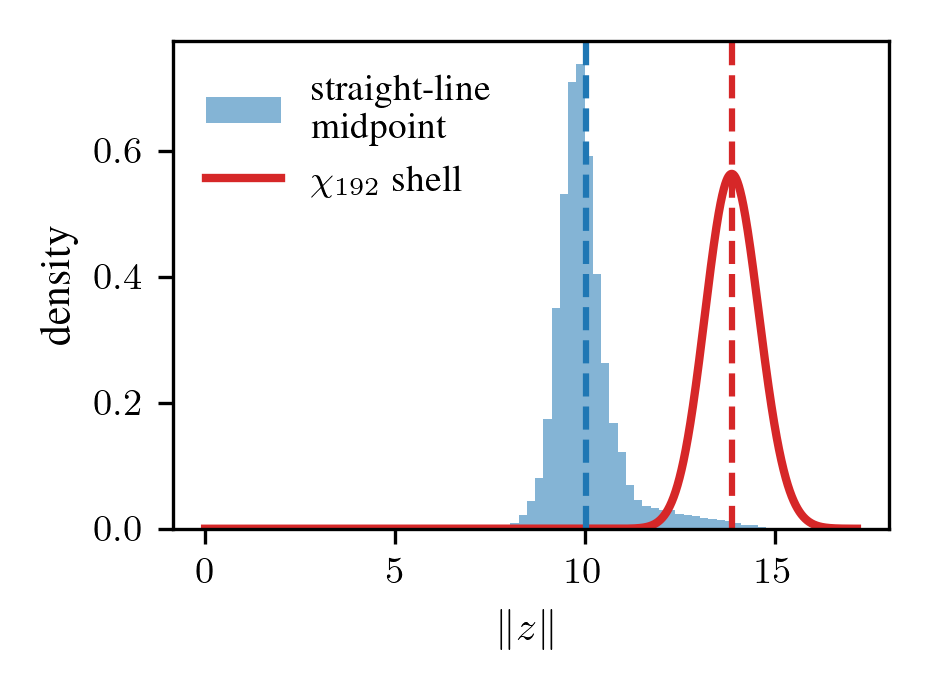
\includegraphics[width=\linewidth]{fig_gaussian_shell_interp_off100_hist}
\begin{minipage}{\linewidth}
\caption{Radii of straight-line latent midpoints for Push-T frame pairs 100 steps apart (blue), with the fitted $\chi_{192}$ shell (red). Most midpoints lie inside the shell. We construct these points by interpolation, without running CEM.}
\label{fig:gaussian-shell-interp}
\end{minipage}
\end{minipage}
\end{figure}
% END inlined content: figure-compute-main.tex

\Cref{thm:graph-progress} explains how repeated calls can make progress when each target
is executable and model, search, and critic errors stay bounded along the route.
Aggregate success rates do not establish those conditions at every call.

\section{Limitations}
\label{sec:limitations}
The critic's labels come from TDR distances, so their accuracy depends on the TDR:
a TDR ball can disagree with the success predicate, and heuristic negatives can mislabel reachable pairs.
Label errors, off-distribution model rollouts, finite action proposals, and
representation aliasing can violate the theoretical error conditions.
The graph links nearby centers and connects the goal using an expanded radius, but these
distances do not ensure feasible transitions. The convergence result assumes local control
and that sufficiently small latent error implies task success. It does not certify the released
checkpoints or prove global convergence of neural training or CEM.

Experiments cover one world-model family and fixed task sets. They do not include matched
runs of SAGE, Hi-LeWM, or ALPS. SAGE reports strong results at offset 150
\citep{sage}, a setting outside our main comparison. We claim neither overall state of the art
nor a general advantage over learned subgoal generators.
The Cube ablations and short-range losses show where the combined objective fails to help.

\section{Conclusion}
Graph-guided terminal costs improve long-horizon and cross-episode planning with a frozen
world model on the evaluated tasks. We bound progress toward graph targets and convergence
near the goal using execution, model, search, and critic errors. These bounds explain
how the method can improve on terminal L2 when suitable action sequences exist and
the controller can find them.
The analysis includes the population normalization scales and the critic in both phases.
It therefore accounts for the critic's effect even after the controller switches to
local L2, when it must reach the goal accurately.

\subsection*{AI use statement}
We used generative AI for literature search, mathematical derivation, proof
checking, manuscript revision, and document-validation scripts. AI assistance did not
produce new benchmark runs; the empirical results are the experimental measurements
reported for this study.

\subsection*{Ethics statement}
The study concerns simulated control benchmarks using public datasets and checkpoints.
It involves no human-subject experiment or sensitive personal data.

\subsection*{Reproducibility statement}
\Cref{app:algorithm,app:hyperparams} specify the planning procedure and reported settings;
\cref{app:render} gives the rendering check. \Cref{app:theory} provides full proofs and
states their assumptions. Mathematical validation examples are separate from benchmark
measurements. Fixed task sets define the evaluation scope; mathematical checks do not
reproduce benchmark runs or establish empirical convergence.

\clearpage
\label{sec:references}
% BEGIN inlined references (edit the bibliography entries here)
\begin{thebibliography}{28}
\providecommand{\natexlab}[1]{#1}
\providecommand{\url}[1]{\texttt{#1}}
\expandafter\ifx\csname urlstyle\endcsname\relax
  \providecommand{\doi}[1]{doi: #1}\else
  \providecommand{\doi}{doi: \begingroup \urlstyle{rm}\Url}\fi

\bibitem[Abate et~al.(2008)Abate, Prandini, Lygeros, and Sastry]{abate2008}
Alessandro Abate, Maria Prandini, John Lygeros, and Shankar Sastry.
\newblock Probabilistic reachability and safety for controlled discrete time
  stochastic hybrid systems.
\newblock \emph{Automatica}, 44\penalty0 (11):\penalty0 2724--2734, 2008.
\newblock \doi{10.1016/j.automatica.2008.03.027}.
\newblock URL
  \url{https://www.cs.ox.ac.uk/people/alessandro.abate/publications/APLS08.pdf}.

\bibitem[Baek et~al.(2025)Baek, Park, Park, Oh, and Kim]{gas}
Seungho Baek, Taegeon Park, Jongchan Park, Seungjun Oh, and Yusung Kim.
\newblock Graph-assisted stitching for offline hierarchical reinforcement
  learning.
\newblock In \emph{International Conference on Machine Learning (ICML)}, 2025.
\newblock URL \url{https://proceedings.mlr.press/v267/baek25a.html}.
\newblock arXiv:2506.07744.

\bibitem[Bertsekas \& Tsitsiklis(1991)Bertsekas and Tsitsiklis]{bertsekas1991}
Dimitri~P. Bertsekas and John~N. Tsitsiklis.
\newblock An analysis of stochastic shortest path problems.
\newblock \emph{Mathematics of Operations Research}, 16\penalty0 (3):\penalty0
  580--595, 1991.
\newblock \doi{10.1287/moor.16.3.580}.
\newblock URL \url{https://www.mit.edu/~jnt/Papers/J034-91-berts-SSP.pdf}.

\bibitem[Caselli et~al.(2026)Caselli, Massafra, Punzo, Lo~Sardo, Pantelidis,
  and Bhethanabhotla]{hilewm}
Niccol\`o Caselli, Francesco Massafra, Samuele Punzo, Salvatore Lo~Sardo,
  Ippokratis Pantelidis, and Sathya~Kamesh Bhethanabhotla.
\newblock Mind the gap: Promises and pitfalls of hierarchical planning in
  {LeWorldModel}.
\newblock \emph{arXiv preprint arXiv:2607.12547}, 2026.
\newblock URL \url{https://arxiv.org/abs/2607.12547}.

\bibitem[Cheng et~al.(2026)Cheng, Zhang, and Wang]{sage}
Letian Cheng, Qi~Zhang, and Yisen Wang.
\newblock {SAGE}: Subgoal-conditioned action generation for latent world model
  planning.
\newblock \emph{arXiv preprint arXiv:2607.17973}, 2026.
\newblock URL \url{https://arxiv.org/abs/2607.17973}.

\bibitem[de~Boer et~al.(2005)de~Boer, Kroese, Mannor, and Rubinstein]{cem}
Pieter-Tjerk de~Boer, Dirk~P. Kroese, Shie Mannor, and Reuven~Y. Rubinstein.
\newblock A tutorial on the cross-entropy method.
\newblock \emph{Annals of Operations Research}, 134\penalty0 (1):\penalty0
  19--67, 2005.
\newblock \doi{10.1007/s10479-005-5724-z}.
\newblock URL
  \url{https://research.utwente.nl/en/publications/a-tutorial-on-the-cross-entropy-method/}.

\bibitem[Emmons et~al.(2020)Emmons, Jain, Laskin, Kurutach, Abbeel, and
  Pathak]{sgm}
Scott Emmons, Ajay Jain, Michael Laskin, Thanard Kurutach, Pieter Abbeel, and
  Deepak Pathak.
\newblock Sparse graphical memory for robust planning.
\newblock In \emph{Advances in Neural Information Processing Systems
  (NeurIPS)}, 2020.
\newblock URL \url{https://arxiv.org/abs/2003.06417}.

\bibitem[Eysenbach et~al.(2019)Eysenbach, Salakhutdinov, and Levine]{sorb}
Benjamin Eysenbach, Ruslan Salakhutdinov, and Sergey Levine.
\newblock Search on the replay buffer: Bridging planning and reinforcement
  learning.
\newblock In \emph{Advances in Neural Information Processing Systems
  (NeurIPS)}, 2019.
\newblock URL \url{https://arxiv.org/abs/1906.05253}.

\bibitem[Gneiting \& Raftery(2007)Gneiting and Raftery]{gneiting2007}
Tilmann Gneiting and Adrian~E. Raftery.
\newblock Strictly proper scoring rules, prediction, and estimation.
\newblock \emph{Journal of the American Statistical Association}, 102\penalty0
  (477):\penalty0 359--378, 2007.
\newblock \doi{10.1198/016214506000001437}.
\newblock URL
  \url{https://sites.stat.washington.edu/people/raftery/Research/PDF/Gneiting2007jasa.pdf}.

\bibitem[Hansen et~al.(2022)Hansen, Wang, and Su]{tdmpc}
Nicklas Hansen, Xiaolong Wang, and Hao Su.
\newblock Temporal difference learning for model predictive control.
\newblock In \emph{International Conference on Machine Learning (ICML)}, 2022.
\newblock URL \url{https://arxiv.org/abs/2203.04955}.

\bibitem[Hansen et~al.(2024)Hansen, Su, and Wang]{tdmpc2}
Nicklas Hansen, Hao Su, and Xiaolong Wang.
\newblock {TD-MPC2}: Scalable, robust world models for continuous control.
\newblock In \emph{International Conference on Learning Representations
  (ICLR)}, 2024.
\newblock URL \url{https://arxiv.org/abs/2310.16828}.

\bibitem[Hoeffding(1963)]{hoeffding1963}
Wassily Hoeffding.
\newblock Probability inequalities for sums of bounded random variables.
\newblock \emph{Journal of the American Statistical Association}, 58\penalty0
  (301):\penalty0 13--30, 1963.
\newblock \doi{10.1080/01621459.1963.10500830}.
\newblock URL
  \url{https://www.tandfonline.com/doi/abs/10.1080/01621459.1963.10500830}.

\bibitem[Hwang et~al.(2026)Hwang, Lee, Kim, and Han]{sse}
Jaebak Hwang, Sanghyeon Lee, Jeongmo Kim, and Seungyul Han.
\newblock Strict subgoal execution: Reliable long-horizon planning in
  hierarchical reinforcement learning.
\newblock In \emph{International Conference on Learning Representations}, 2026.
\newblock URL \url{https://arxiv.org/abs/2506.21039}.

\bibitem[Janner et~al.(2019)Janner, Fu, Zhang, and Levine]{mbpo}
Michael Janner, Justin Fu, Marvin Zhang, and Sergey Levine.
\newblock When to trust your model: Model-based policy optimization.
\newblock In \emph{Advances in Neural Information Processing Systems},
  volume~32, 2019.
\newblock URL
  \url{https://proceedings.neurips.cc/paper/2019/hash/5faf461eff3099671ad63c6f3f094f7f-Abstract.html}.

\bibitem[Kostrikov et~al.(2022)Kostrikov, Nair, and Levine]{iql}
Ilya Kostrikov, Ashvin Nair, and Sergey Levine.
\newblock Offline reinforcement learning with implicit {Q}-learning.
\newblock In \emph{International Conference on Learning Representations}, 2022.
\newblock URL \url{https://arxiv.org/abs/2110.06169}.

\bibitem[Koul et~al.(2024)Koul, Sujit, Chen, Evans, Wu, Xu, Chari, Islam,
  Seraj, Efroni, Molu, Dud\'{\i}k, Langford, and Lamb]{pclast}
Anurag Koul, Shivakanth Sujit, Shaoru Chen, Ben Evans, Lili Wu, Byron Xu, Rajan
  Chari, Riashat Islam, Raihan Seraj, Yonathan Efroni, Lekan~P Molu, Miroslav
  Dud\'{\i}k, John Langford, and Alex Lamb.
\newblock {PcLast}: Discovering plannable continuous latent states.
\newblock In \emph{International Conference on Machine Learning}, pp.\
  25475--25493, 2024.
\newblock URL \url{https://proceedings.mlr.press/v235/koul24a.html}.

\bibitem[Li et~al.(2026{\natexlab{a}})Li, Wang, Qiu, Xiong, and Liu]{trm}
Liangyu Li, Shengzhi Wang, Libin Qiu, Mingliang Xiong, and Qingwen Liu.
\newblock World model control by trajectory reachability metrics.
\newblock \emph{arXiv preprint arXiv:2605.22164}, 2026{\natexlab{a}}.
\newblock URL \url{https://arxiv.org/abs/2605.22164}.

\bibitem[Li et~al.(2026{\natexlab{b}})Li, Li, Maeda, Ogawa, and
  Haseyama]{rcaux}
Wenyuan Li, Guang Li, Keisuke Maeda, Takahiro Ogawa, and Miki Haseyama.
\newblock Predictive but not plannable: {RC-aux} for latent world models.
\newblock \emph{arXiv preprint arXiv:2605.07278}, 2026{\natexlab{b}}.
\newblock URL \url{https://arxiv.org/abs/2605.07278}.

\bibitem[Lowrey et~al.(2019)Lowrey, Rajeswaran, Kakade, Todorov, and
  Mordatch]{polo}
Kendall Lowrey, Aravind Rajeswaran, Sham Kakade, Emanuel Todorov, and Igor
  Mordatch.
\newblock Plan online, learn offline: Efficient learning and exploration via
  model-based control.
\newblock In \emph{International Conference on Learning Representations
  (ICLR)}, 2019.
\newblock URL \url{https://arxiv.org/abs/1811.01848}.

\bibitem[Maes et~al.(2026)Maes, Le~Lidec, Scieur, LeCun, and Balestriero]{lewm}
Lucas Maes, Quentin Le~Lidec, Damien Scieur, Yann LeCun, and Randall
  Balestriero.
\newblock {LeWorldModel}: Stable end-to-end joint-embedding predictive
  architecture from pixels.
\newblock \emph{arXiv preprint arXiv:2603.19312}, 2026.
\newblock URL \url{https://arxiv.org/abs/2603.19312}.

\bibitem[Mayne et~al.(2000)Mayne, Rawlings, Rao, and Scokaert]{mayne2000}
David~Q. Mayne, James~B. Rawlings, Christopher~V. Rao, and Pierre O.~M.
  Scokaert.
\newblock Constrained model predictive control: Stability and optimality.
\newblock \emph{Automatica}, 36\penalty0 (6):\penalty0 789--814, 2000.
\newblock \doi{10.1016/S0005-1098(99)00214-9}.
\newblock URL
  \url{https://www.sciencedirect.com/science/article/pii/S0005109899002149}.

\bibitem[Newey \& Powell(1987)Newey and Powell]{newey1987}
Whitney~K. Newey and James~L. Powell.
\newblock Asymmetric least squares estimation and testing.
\newblock \emph{Econometrica}, 55\penalty0 (4):\penalty0 819--847, 1987.
\newblock \doi{10.2307/1911031}.
\newblock URL \url{https://www.jstor.org/stable/1911031}.

\bibitem[Park et~al.(2024)Park, Kreiman, and Levine]{hilp}
Seohong Park, Tobias Kreiman, and Sergey Levine.
\newblock Foundation policies with {Hilbert} representations.
\newblock In \emph{International Conference on Machine Learning (ICML)}, 2024.
\newblock URL \url{https://proceedings.mlr.press/v235/park24g.html}.

\bibitem[Park et~al.(2025)Park, Frans, Eysenbach, and Levine]{ogbench}
Seohong Park, Kevin Frans, Benjamin Eysenbach, and Sergey Levine.
\newblock {OGBench}: Benchmarking offline goal-conditioned {RL}.
\newblock In \emph{International Conference on Learning Representations
  (ICLR)}, 2025.
\newblock URL \url{https://arxiv.org/abs/2410.20092}.

\bibitem[Savinov et~al.(2018)Savinov, Dosovitskiy, and Koltun]{sptm}
Nikolay Savinov, Alexey Dosovitskiy, and Vladlen Koltun.
\newblock Semi-parametric topological memory for navigation.
\newblock In \emph{International Conference on Learning Representations
  (ICLR)}, 2018.
\newblock URL \url{https://arxiv.org/abs/1803.00653}.

\bibitem[Shehmar et~al.(2026)Shehmar, Schlegel, Taylor, and Machado]{alps}
Dikshant Shehmar, Matthew Schlegel, Matthew~E. Taylor, and Marlos~C. Machado.
\newblock Laplacian representations for decision-time planning.
\newblock In \emph{International Conference on Machine Learning}, 2026.
\newblock URL \url{https://arxiv.org/abs/2602.05031}.

\bibitem[Wang et~al.(2023)Wang, Torralba, Isola, and Zhang]{qrl}
Tongzhou Wang, Antonio Torralba, Phillip Isola, and Amy Zhang.
\newblock Optimal goal-reaching reinforcement learning via quasimetric
  learning.
\newblock In \emph{International Conference on Machine Learning (ICML)}, 2023.
\newblock URL \url{https://arxiv.org/abs/2304.01203}.

\bibitem[Zhou et~al.(2024)Zhou, Pan, LeCun, and Pinto]{dinowm}
Gaoyue Zhou, Hengkai Pan, Yann LeCun, and Lerrel Pinto.
\newblock {DINO-WM}: World models on pre-trained visual features enable
  zero-shot planning.
\newblock \emph{arXiv preprint arXiv:2411.04983}, 2024.
\newblock URL \url{https://arxiv.org/abs/2411.04983}.

\end{thebibliography}
% END inlined references
\clearpage
\appendix
% BEGIN inlined content: theory-appendix.tex
\section{Detailed theory and proofs}
\label{app:theory}

\subsection{Scope, state, and time conventions}
\label{app:theory-setup}
We hold the trained encoder, predictor, TDR, graph, and critic fixed throughout the analysis.
We examine whether the controller reduces the remaining graph distance, whether this
progress brings it to a region where local control reaches the goal, and when the
critic's score measures an expected time to reach the goal.
Graph connectivity alone does not establish these properties.
All error tolerances and optimization gaps below are nonnegative; the graph radius,
lookahead, and normalization floors are positive.

Let $x$ denote a physical state, or a history state sufficient to make the dynamics
Markov. Write $z(x)$ for its current encoded observation and
$\psi(x)=\psi(z(x))$ when no confusion results. The LeWM predictor uses
its input history as well as its current latent. In the deterministic results,
$x^+(u)$ is the state after the entire sequence $u$ of $L=K\Delta$ primitive actions,
and $z^+(u)=z(x^+(u))$. Write $\hat z^+(u)$ for the predicted endpoint.
We bound prediction error for the observed input history.
The graph-descent theorem therefore does not require a single image latent to be Markov.
The Bellman results require a state that contains enough information to be Markov.
If the implemented critic receives only $z(x)$, its error must include information lost
by that input restriction.

Fix a goal observation $z_g$. Let $\mathcal G_g$ be the measurable set of environment
states that satisfy the task's goal condition. Raw latent distance to $z_g$ need not identify this set.
For example, a goal may constrain only an object's position while images also contain
an unconstrained robot configuration. Conversely, two identical rendered arm poses can
have different unwrapped joint coordinates. The local theorem explicitly assumes that a
small enough latent error implies task success. Matching goal images alone does not
ensure that every environment's goal condition holds.
When the agent satisfies the goal condition, the controller ends the episode and skips
any remaining actions in the current plan.
We need endpoint bounds only for calls that have not already reached the goal.
If the agent reaches the goal during a call, it has already satisfied the theorem's
conclusion, even if its latent lies outside the TDR switching region.
The graph phase therefore ends when the agent first reaches the goal or enters $\Rset$.

\begin{definition}[Block hitting time]
Under continuation policy $\pi$, let $\tau^\pi$ be the first environment step at which
the agent enters $\mathcal G_g$, with value $\infty$ if it never enters. Define
$T^\pi=\Delta\lceil\tau^\pi/\Delta\rceil$, including $T^\pi=0$ for an initially
successful state. The block process records whether success occurred at any time within
a block and makes that event absorbing.
\end{definition}
We count the first time the agent satisfies the goal condition as success; the
physical object need not remain at the goal afterward.
A block transition that inspects only its final image may miss an earlier success.
Such an omission is a modeling error when the intended labels record first hits.
The state in the Bellman analysis includes the hit flag when it is needed.

All empirical budgets are in primitive environment steps. The critic grid has spacing
$\Delta=5$, the MPC horizon is $K=5$ blocks, and the controller executes up to $L=25$
steps per call, stopping early if it reaches the goal.
The main protocols have budgets divisible by $L$. If the remaining budget is smaller
than $L$, the controller must shorten the plan and update the clock by the number of
executed steps, or stop. The full-$L$ formulas apply only when at least $L$ steps remain.
We learn the discounted TDR from consecutive-frame transitions; it has its own
calibrated units. Neither $\Htd$ nor $\lambda$ is itself a count of environment steps.

\paragraph{Relationship to earlier guarantees.}
The representation theorem in HILP links embedding and directional-action error to
optimal goal-reaching under its stated deterministic assumptions \citep{hilp}.
Our controller instead tracks a node chosen by graph search and executes a whole action
sequence. The proof below works with the finite graph's actual path length, without
assuming a globally accurate embedding of optimal temporal distance.
PcLast and ALPS use learned representations for hierarchical model-based planning
\citep{pclast,alps}; the spectral commute-time identity in ALPS concerns representation
geometry, whereas we bound progress under the controller's combined cost.
The terminal proof uses the local contraction structure familiar from MPC
\citep{mayne2000}. The reachability recursion is a finite-horizon dynamic program
\citep{abate2008},
which uses different assumptions from infinite-horizon stochastic shortest-path convergence
\citep{bertsekas1991}.

\paragraph{Correspondence between the algorithm and the assumptions.}
The potential in \cref{eq:potential} is the start-attachment objective in
\cref{eq:startnode}, using the stored TDR centers and the same fixed goal graph.
The path length includes the start attachment, as the algorithm's lookahead rule requires.
The comparison sequence contains $K$ action blocks. We compare the frozen predictor's
endpoint with the endpoint after executing all $L$ steps. This assumption requires a
suitable action sequence, without requiring a learned low-level policy.
We score CEM's returned mean and the comparison sequence using the final population's
normalization constants. We do not recompute the IQR after adding either sequence.
Earlier CEM iterations may use different constants; the proof compares both sequences
under the same final objective.

The critic remains in the cost after the local switch, so differences in its scores contribute
to both \cref{eq:rho,eq:local-floor}. The Bellman reference allows feedback between
$\Delta$-step blocks, whereas the controller commits to $K$ such blocks; an accurate
reference critic is therefore not automatically the value of this controller.
The common-policy survival interpretation requires a separately specified continuation
policy. Finally, the tabular expectile theorem analyzes exact value-table updates.
TDR training instead uses twin networks, lagged targets, and Euclidean distances.
The main progress theorem treats the trained representation as fixed and does not
require its optimizer to converge.

If a variant scores the mapped medoid $\tilde y_q=\psi(z_q)$ instead of the graph
center $y_q$, let $\delta_q=\|\tilde y_q-y_q\|$.
If the comparison sequence ends within $\eta$ of $\tilde y_q$, the same argument bounds
the executed endpoint's distance to the graph center by $\rho+\delta_q$; use that
quantity in the radius and descent conditions. If $\eta$ instead measures the
comparison sequence's endpoint distance to $y_q$, use $\rho+2\delta_q$.
Both statements follow by one triangle inequality at each changed target comparison.
Replacing centers by medoids therefore changes the error bound; the formulas must
account for the distance between the two targets.

\subsection{Restricted attachment and path progress}
\label{app:graph-proof}
Let $G_g$ be a finite graph augmented by the goal node, with coordinate $y_g=\psi(z_g)$.
Its edges have nonnegative weights equal to Euclidean distances between their coordinates.
$D_g[v]$ is finite only for nodes connected to the goal. Choose shortest paths without
repeated nodes; such paths exist even with zero-weight edges. Define
\[
 A(z)=\{v\in V_G:\|\psi(z)-y_v\|\le\Htd,\ D_g[v]<\infty\}.
\]
The goal is not needed as an extra member of $A(z)$: the explicit local switch handles
states near it. If $A(z)$ is empty, $\Phi(z)=+\infty$, and no finite graph-progress bound
applies. The following results assume that at least one attachment has a finite route to the goal.

\begin{lemma}[Path prefix and attachment]
\label{lem:path-prefix}
Let $v^\star$ attain \cref{eq:potential}, and let $q$ be a node on a selected shortest
path from that attachment to the goal. Let $p_q$ be the cumulative path length from
$\psi(z)$ to $y_q$, including the initial attachment segment. Then
\begin{equation}
 \Phi(z)=p_q+D_g[q],\qquad
 \dd(z,z_g)\le\Phi(z).
 \label{eq:prefix-identity}
\end{equation}
Here $D_g[g]=0$. If $q$ is a regular graph node and
$\|\psi(z')-y_q\|\le\Htd$, then
\begin{equation}
 \Phi(z')\le\Phi(z)-p_q+\|\psi(z')-y_q\|.
 \label{eq:reattach}
\end{equation}
\end{lemma}
\begin{proof}
Every suffix of the selected shortest path is a shortest path from its initial node
to the goal. Otherwise replacing that suffix with a shorter one would shorten the
selected path. Its total length, including the attachment cost, is $\Phi(z)$, which
proves the first identity. Applying the Euclidean triangle inequality successively to
the coordinates along the same path proves the second inequality. If the displayed
distance from $z'$ to $q$ is at most $\Htd$, the node $q$ is a feasible member of $A(z')$:
it has finite $D_g[q]$ because it lies on the route. Evaluating the minimum defining
$\Phi(z')$ at $q$ proves \cref{eq:reattach}.
\end{proof}

The proof does not assume that $D_g$ has a Lipschitz extension or that $\Phi$ is continuous.
The radius restriction can make $\Phi$ jump when a node enters or leaves the attachment
set. We therefore require the next endpoint to lie within $\Htd$ of the selected node.
A qualitative statement that the endpoint is nearby would not suffice.

\begin{lemma}[First-crossing lookahead]
\label{lem:overshoot}
Suppose $z\notin\Rset$. The selected path has length greater than $\lambda$ and
therefore contains a first $\lambda$-crossing target. If $r_e$ is the largest segment
on the augmented path, including the initial attachment, then
\[
 \lambda\le p_q<\lambda+r_e .
\]
One may take $r_e\le\max(\Htd,r_g)$ for the stated graph construction.
\end{lemma}
\begin{proof}
By \cref{lem:path-prefix}, $\Phi(z)\ge\dd(z,z_g)>\lambda$.
The finite cumulative sequence starts at zero and ends at $\Phi(z)$.
Just before its first crossing it is strictly below $\lambda$; the crossing adds
one segment of length at most $r_e$. Regular edges and the initial attachment are at
most $\Htd$, and goal-attachment edges are at most $r_g$.
\end{proof}
The selected target can therefore lie beyond the calibrated lookahead distance.
In particular, expanding the goal-attachment radius can create a much longer last edge.
The comparison sequence in \cref{thm:graph-progress} must reach near this actual target,
including any extra distance from crossing the lookahead threshold.
Likewise, resetting cluster centers to means after sequential admission does not
preserve an admission-radius guarantee for all members. The proof needs the actual
center distances and endpoint error, not an unproved bound on cluster radii.

\begin{lemma}[Graph descent from endpoint tracking]
\label{lem:tracking-descent}
Suppose a first-crossing target is tracked with error
$\|\psi(z')-y_q\|\le\rho$, where $\rho\le\Htd$ and $\rho<\lambda$.
Then either $z'\in\Rset$ or
$\Phi(z')\le\Phi(z)-\lambda+\rho$.
\end{lemma}
\begin{proof}
If $q$ is regular and $z'$ is outside $\Rset$, apply \cref{lem:path-prefix} and
$p_q\ge\lambda$. If $q=g$, the tracking error is
$\dd(z',z_g)\le\rho<\lambda$, so $z'\in\Rset$. These cases exhaust the possibilities.
\end{proof}

\paragraph{Why geometric edges require an execution assumption.}
An undirected radius graph can connect two latent clusters even if the physical
dynamics permit travel in only one direction, or no travel at all.
The temporal-efficiency filter concerns observed directions within episodes and does
not prove reversibility of arbitrary inter-cluster edges.
A finite $D_g$ therefore does not ensure that the agent can follow the route.
The comparison-sequence assumption requires an executable plan to the chosen target.
It allows other graph edges to be infeasible, but requires more than proximity between
the current state and target coordinates.

\subsection{The normalized CEM cost and execution error}
\label{app:cost-proof}
Fix one planning call, target, horizon grid, and set of normalization constants.
Write
\[
 \widehat b(u)=\|\psi(\hat z^+(u))-y_q\|,\quad
 \widehat S(u)=\Delta\sum_{j=0}^{n}[1-V(\hat z^+(u),z_g,j\Delta)].
\]
Since the critic outputs lie in $[0,1]$, $0\le\widehat S(u)\le C_n$ even if they are
not monotone in the horizon. Denote the two population medians by $m_b,m_S$.

\begin{lemma}[Exact scale-ratio comparison]
\label{lem:normalized}
If
\[
 \frac{\widehat b(\hat u)-m_b}{s_b}
 +\beta\frac{\widehat S(\hat u)-m_S}{s_S}
 \le
 \frac{\widehat b(u^\circ)-m_b}{s_b}
 +\beta\frac{\widehat S(u^\circ)-m_S}{s_S}
 +\epsilon_{\mathrm{opt}},
\]
with $s_b,s_S>0$ and $\beta\ge0$, then
\begin{equation}
 \widehat b(\hat u)\le\widehat b(u^\circ)
       +s_b\epsilon_{\mathrm{opt}}
       +\beta\frac{s_b}{s_S}
                    [\widehat S(u^\circ)-\widehat S(\hat u)]_+ .
 \label{eq:scale-comparison}
\end{equation}
\end{lemma}
\begin{proof}
Cancel the medians, move the critic difference to the right, and multiply by $s_b$.
Replacing a negative critic difference by zero can only enlarge the right side.
\end{proof}
Normalization still leaves a tradeoff between the two costs.
For example, multiplying raw critic scores by a positive constant generally cancels
through their IQR when the floor is inactive, but a very small critic IQR can amplify
small, unreliable variations. The numerical floors make the objective defined; they
do not establish that the resulting scale ratio is appropriate.
If two candidates use different population medians or scales, those constants do not
cancel and the comparison above no longer applies.

\begin{proof}[Proof of \cref{thm:graph-progress}]
If the agent reaches the goal before the call ends, the conclusion already holds.
Otherwise,
the triangle inequality and the model-error assumption give
\[
 \widehat b(u^\circ)\le
 \|\psi(z^+(u^\circ))-y_q\|
 +\|\psi(\hat z^+(u^\circ))-\psi(z^+(u^\circ))\|
 \le\eta+e_\psi .
\]
Apply \cref{lem:normalized}, then bound the distance between the predicted and true
endpoints of the returned sequence:
\begin{align*}
 \|\psi(z^+(\hat u))-y_q\|
 &\le\widehat b(\hat u)+e_\psi\\
 &\le\eta+2e_\psi+s_b\epsilon_{\mathrm{opt}}
                +\beta(s_b/s_S)\omega=\rho.
\end{align*}
\Cref{lem:tracking-descent} proves the one-call claim.
For the iteration bound, let $\tau_G$ be the first call that reaches the goal or has
an endpoint in $\Rset$, and let
$a_G=\lambda-\rho>0$. If $\tau_G>N$,
all of the first $N$ transitions remain outside $\Rset$, so induction gives
$0\le\Phi(z_N)\le\Phi(z_0)-Na_G$.
For $N=\lceil\Phi(z_0)/a_G\rceil$, the right side is nonpositive.
Equality is also impossible outside $\Rset$, since
$\Phi(z_N)\ge\dd(z_N,z_g)>\lambda>0$.
Thus $\tau_G\le N$. If the initial state is already successful or in $\Rset$, take $N_G=0$.
\end{proof}

\paragraph{What the optimization assumption means for CEM.}
The comparison need not assume a global minimizer.
It can use any feasible sequence $u^\circ$ whose tracking error is controlled,
provided the returned sequence has the stated objective gap relative to that sequence.
CEM's final mean is not necessarily a sampled candidate or an elite, and a mean of
successful sequences can fail in a nonlinear system. Therefore a proof concerning only
the best elite would not prove the theorem for the stated implementation.
Here $\epsilon_{\mathrm{opt}}$ compares the sequence the controller actually executes
with the feasible comparison sequence, using the final population's fixed constants.
Thirty CEM iterations do not establish that this gap is small
\citep{cem}. One could evaluate the returned mean and retain a candidate with a lower
score. The reported runs do not establish that they used this additional check.

\begin{proposition}[Action coverage under adaptive sampling]
\label{prop:coverage}
Let $\mathcal U_\eta$ be sequences meeting a prescribed true tracking tolerance.
Suppose every conditional CEM proposal, given all previous draws, places probability
at least $p>0$ on $\mathcal U_\eta$. Among $N$ draws the probability of seeing no such
sequence is at most $(1-p)^N$.
\end{proposition}
\begin{proof}
Let $F_i$ be the event that the first $i$ proposals miss $\mathcal U_\eta$.
Conditional on the past and $F_{i-1}$, the next failure probability is at most $1-p$.
The tower property yields $\PP(F_i)\le(1-p)\PP(F_{i-1})$.
Induction proves the result; independence between iterations is not required.
\end{proof}
This result bounds the chance of sampling a useful sequence under the stated coverage assumption.
If CEM concentrates its Gaussian proposals too narrowly, the lower bound $p$ may fail.
Even when CEM samples a good sequence, its final mean need not be good.
Retrieval changes which actions CEM is likely to sample. It can therefore help
independently of the cost, as the Cube results suggest.

\paragraph{Prediction error over one planning call.}
Suppose true and predicted histories admit a common normed state
space with block transitions $f$ and $\hat f$, the initial history error is zero, and
\[
 \|\hat f(x,a)-f(x,a)\|\le\varepsilon_P,\qquad
 \|f(x,a)-f(x',a)\|\le L_f\|x-x'\|
\]
on all compared rollout states and actions. Applying both transitions to the same
action sequence and using induction gives
\begin{equation}
 e_K\le\varepsilon_P\sum_{i=0}^{K-1}L_f^i .
 \label{eq:rollout-error}
\end{equation}
Indeed $e_{k+1}\le\varepsilon_P+L_fe_k$ by adding and subtracting the true transition
from the predicted state. If the map from history to the endpoint TDR coordinate
is $L_\psi$-Lipschitz, take $e_\psi\le L_\psi e_K$.
The bound is $K\varepsilon_P$ for $L_f=1$, is bounded uniformly in $K$ for
$L_f<1$, and can grow geometrically for $L_f>1$.
These assumptions suffice to bound endpoint error. A small latent prediction loss
alone does not imply them, especially if the encoded history cannot determine the next state.
The graph supports progress across many short calls, while this model bound covers
only one call. Model-based RL analyses also use short rollouts to limit accumulated
error \citep{mbpo}. Here we do not assume globally stable LeWM dynamics.
Each replan starts from new observations, but the endpoint bound must still hold
at every state the controller reaches.

\subsection{Terminal-region convergence and the complete budget}
\label{app:local-proof}
The switched branch uses squared raw latent distance, while the graph branch uses an
unsquared TDR distance. The distinction changes the optimization-error term from
linear to square-root dependence.
We include the critic in the local-phase proof because the controller still uses it.

\begin{proof}[Proof of \cref{thm:local}]
If a call succeeds before its endpoint, the success conclusion already holds.
At a local state of error $e$, let $u^\circ$ be the contracting comparison sequence.
Its true endpoint error is at most $ae$, and its predicted endpoint error is at most
$ae+e_z$. \Cref{lem:normalized}, now applied to the squared base cost, gives
\[
 \|\hat z^+(\hat u)-z_g\|^2
 \le (ae+e_z)^2+
       s_b\epsilon_{\mathrm{opt}}+\beta(s_b/s_S)\omega_\ell.
\]
All terms added on the right are nonnegative. Taking square roots and using
$\sqrt{v^2+w}\le v+\sqrt w$ for $v,w\ge0$, followed by the endpoint model bound,
yields
\[
 e(z^+(\hat u))
 \le ae+2e_z+
       \sqrt{s_b\epsilon_{\mathrm{opt}}+\beta(s_b/s_S)\omega_\ell}
 =ae+d_\ell .
\]
Invariance ensures that the next call again uses this branch and its assumptions.
Iteration gives
$e(z_m)\le a^m e(z_0)+d_\ell\sum_{i=0}^{m-1}a^i
\le a^mR+(1-a^m)e_\infty$.
It suffices that $a^mR\le r_{\mathrm{goal}}-e_\infty$, which is precisely the
stated conservative bound on $m$. If $R=0$, entry is already successful.
The assumption that latent error within $r_{\mathrm{goal}}$ implies task success proves the claim.
Adding the graph and local call counts proves the execution-budget bound.
Reaching the goal during either phase only shortens the execution.
\end{proof}

\paragraph{Ensuring that the controller stays in the local region.}
One sufficient special case is that, on a local domain,
$\Rset=\{z:e(z)\le R\}$ and $aR+d_\ell\le R$.
The contraction inequality then leaves the state in $\Rset$.
More generally, each local call must end inside the TDR switching region until success.
Small raw latent error alone does not ensure this; one must relate raw latent distance
to TDR distance.
If the implemented controller exits $\Rset$, the local proof stops and the graph
phase can resume. Neither theorem alone rules out repeated switching.
The assumption that local calls stay in the region is therefore necessary for this proof.

\paragraph{Success tolerance and an unavoidable error floor.}
With persistent model or optimization error, the bound approaches $e_\infty$ rather
than zero. The strict condition $e_\infty<r_{\mathrm{goal}}$ ensures that the error bound
eventually enters the success tolerance. If $e_\infty=r_{\mathrm{goal}}$ and $R$ is larger,
the upper bound approaches the boundary without reaching it in finite time.
If unsuccessful states can lie arbitrarily close to the goal latent, no positive
latent radius guarantees task success. This matters when the goal depends on
state coordinates that the image does not reveal.

\paragraph{Clock dependence and available time.}
The ET grid and its IQR change with $B-t-L$.
To combine \cref{thm:local,thm:graph-progress}, choose error constants that cover every
call at its remaining budget. Values measured only at the initial budget need not suffice.
If $B<L(N_G+N_\ell)$ the theorem does not assert success within the episode,
although the controller may succeed faster than the bound.
Increasing the number of steps executed before replanning requires a new model-error bound.

\subsection{Stochastic execution and expected progress}
\label{app:stochastic}
We now allow individual calls to violate the deterministic assumptions with bounded probability.
The first result bounds success probability within a fixed budget by bounding the chance
of any such violation. The second bounds the expected number of graph calls and also
requires a limit on how much a failed call can increase the remaining distance.

\begin{corollary}[Finite-budget success event]
\label{cor:high-prob}
Let $N=N_G+N_\ell$ bound the number of calls whenever all deterministic assumptions hold.
Conditional on earlier calls satisfying their bounds and on their history, suppose
call $j$ obeys the appropriate one-call error and comparison bounds with probability
at least $1-p_j$. Include the bound $e\le R$ on local entry and retention in $\Rset$
for local calls that do not succeed. Take $0\le p_j\le1$.
If $B\ge LN$, success probability is at least
$1-\sum_{j=1}^{N}p_j$ (or zero when that lower bound is negative).
\end{corollary}
\begin{proof}
The probability that the first violated call occurs at $j$ is at most $p_j$,
by conditioning on the history up to that call.
These first-failure events are disjoint. On their complement the deterministic
bound applies for all required calls. Summing their probabilities proves
the lower bound. Once the agent reaches the goal, no later call can fail because the
episode has ended. The proof does not require independence between calls.
\end{proof}
An ensemble standard deviation alone does not give the $p_j$ values.
To apply the corollary, one must justify the conditional execution or model-error
probabilities separately; the corollary then combines them.

\begin{proposition}[Expected graph-phase duration]
\label{prop:drift}
Let $\tau_G$ be the first call with success or local-region entry, and set
$W_j=\Phi(z_j)$ before $\tau_G$ and $W_j=0$ afterward, for a fixed initial state.
Assume these stopped potentials are finite and integrable.
Before $\tau_G$, suppose a good call decreases $W$ by at least $a_G>0$ with conditional
probability at least $1-p$, while any other call increases it by at most $M$.
Here $0\le p\le1$ and $M\ge0$.
If $\delta=(1-p)a_G-pM>0$, then $\tau_G$ satisfies
\[
 \EE[\tau_G]\le W_0/\delta.
\]
\end{proposition}
\begin{proof}
For $j<\tau_G$, the conditional expected increment is at most
$-(1-p)a_G+pM=-\delta$. After stopping the increment is zero. Hence
\[
 \EE W_{(n+1)\wedge\tau_G}
 \le \EE W_{n\wedge\tau_G}-\delta\,\PP(\tau_G>n).
\]
Sum for $n=0,\ldots,m-1$ and use nonnegativity of the left-hand potential:
$\delta\sum_{n=0}^{m-1}\PP(\tau_G>n)\le W_0$.
Monotone convergence and the integer tail-sum identity give the result.
\end{proof}
For the deterministic progress bound, $a_G=\lambda-\rho\le\lambda$.
Reaching the goal or entering $\Rset$ also gives the required decrease: outside that set
$\Phi(z)>\lambda\ge a_G$, so resetting $W$ to zero decreases it by at least $a_G$.
If a failed call can lose all finite graph attachments, no finite $M$ follows.
This result therefore does not cover calls that disconnect the agent from the goal graph.

\subsection{What the survival score measures}
\label{app:survival}
For a specified policy $\pi$, write
$F_j^\pi(x)=\PP_x^\pi(T^\pi\le j\Delta)$ and
$S_n^\pi(x)=\Delta\sum_{j=0}^{n}(1-F_j^\pi(x))$.
The probabilities are nondecreasing in $j$ because the underlying first-hit events
are nested.

\begin{proposition}[Survival identity, truncation, and ranking]
\label{prop:survival}
For any such policy, including one with a positive probability of never hitting,
\begin{equation}
 S_n^\pi(x)=\EE_x^\pi[\min(T^\pi,C_n)],\qquad C_n=(n+1)\Delta.
 \label{eq:tail-identity}
\end{equation}
If $F_j^a\ge F_j^b$ for every queried $j$, then $S_n^a\le S_n^b$.
If one inequality is strict, the score inequality is strict.
Two states with the same final-deadline probability can nevertheless have different
$S_n$.
\end{proposition}
\begin{proof}
For every $T\in\{0,\Delta,2\Delta,\ldots,\infty\}$, the pointwise identity
\[
 \min(T,(n+1)\Delta)=\Delta\sum_{j=0}^{n}\ind_{\{T>j\Delta\}}
\]
counts the grid intervals before truncation. Because the sum is finite, we can take
expectations term by term even when $\EE T$ is infinite. This proves the
first claim. Subtracting the sums proves the dominance statements.
For the last claim, take deterministic times $\Delta$ and $2\Delta$ with $n\ge2$:
both final probabilities are one but their scores are $\Delta$ and $2\Delta$.
\end{proof}

\paragraph{The endpoint convention.}
The grid $j=0,\ldots,n$ includes a term at the final queried deadline $n\Delta$.
Truncating the hitting time at that deadline would require summing only
$j=0,\ldots,n-1$, giving zero when $n=0$.
Our score retains the last term and therefore has cap $C_n$.
At zero remaining time, it is $\Delta(1-V_0)$, an endpoint-success penalty.
At the maximum query horizon of 50 steps it has cap 55 steps.
This extra interval changes rankings whenever $V_n$ differs across candidates;
so removing it can change which candidate the planner prefers.

If $\tau^\pi$ is the primitive hitting time, rounding introduces a bounded discrepancy:
for any grid-aligned cap $C$,
\[
 0\le
 \EE\min(\Delta\lceil\tau^\pi/\Delta\rceil,C)
       -\EE\min(\tau^\pi,C)
 \le\Delta.
\]
This follows pointwise from $0\le\Delta\lceil\tau/\Delta\rceil-\tau<\Delta$ at
finite $\tau$, with both capped quantities equal at $\tau=\infty$.
Even with exact grid probabilities, the score measures time rounded up to the next
block boundary, with the discrepancy bounded above.

\begin{proposition}[Horizon-wise optima and policy consistency]
\label{prop:policy-consistency}
Let $\Pi$ be a common policy class and
$V_j^*(x)=\sup_{\pi\in\Pi}F_j^\pi(x)$.
Define
\[
 S_n^*(x)=\Delta\sum_{j=0}^{n}(1-V_j^*(x)),\qquad
 C_n^*(x)=\inf_{\pi\in\Pi}S_n^\pi(x).
\]
Then $S_n^*\le C_n^*$ and, with $A_\pi=\Delta\sum_{j=0}^{n}(V_j^*-F_j^\pi)$,
\begin{equation}
 C_n^*-S_n^*=\inf_{\pi\in\Pi} A_\pi\ge0.
 \label{eq:consistency-gap}
\end{equation}
Equality holds if a single policy achieves all the horizon optima.
More generally, if some $\bar\pi$ satisfies
$0\le V_j^*-F_j^{\bar\pi}\le a_j$, then
$0\le C_n^*-S_n^*\le\Delta\sum_{j=0}^{n}a_j$.
\end{proposition}
\begin{proof}
For every fixed $\pi$, subtract the finite sums to obtain
$S_n^\pi=S_n^*+A_\pi$. Each summand in $A_\pi$ is nonnegative.
Taking the infimum proves the identity and lower bound. Substituting a jointly
optimal policy, or the approximate policy $\bar\pi$, gives the remaining claims.
An infimum need not be attained for the identity to hold.
\end{proof}

\paragraph{A strict policy-consistency gap.}
Take $\Delta=1$, $n=2$, and an initial state with two irreversible choices.
Choice A reaches the goal at time 1 with probability 0.6 and never reaches it otherwise.
Choice B reaches the goal at time 2 with certainty. There are no later choices.
Then $V_0^*=0$, $V_1^*=0.6$, and $V_2^*=1$, so $S_2^*=1.4$.
Policy A has truncated expectation $0.6\cdot1+0.4\cdot3=1.8$;
policy B has expectation 2. Randomizing between them gives a convex combination,
so $C_2^*=1.8>S_2^*$.
The values $j\mapsto V_j^*$ never decrease with the horizon and define a valid cumulative
distribution on this grid. Yet no policy in this example has that hitting-time distribution.
A critic can therefore be nondecreasing in the horizon without describing any single policy.

\paragraph{Expected truncated time is not deadline success.}
Even with a common policy interpretation, minimizing the score is not equivalent to
maximizing probability of success by the final deadline.
With deadline 5 and cap 6, one choice hits at time 1 with probability 0.49 and never
hits otherwise; another hits at time 5 with certainty.
Their scores are $0.49+0.51\cdot6=3.55$ and 5, respectively.
The score prefers the less reliable choice because it assigns enough value to early success.
Minimizing this cost therefore does not impose a lower bound on the probability of
success by the deadline.

\begin{corollary}[Clock sensitivity]
\label{cor:clock}
For $n'\ge n$ and any $[0,1]$-valued horizon predictions,
\[
 0\le \widehat S_{n'}(x)-\widehat S_n(x)\le\Delta(n'-n).
\]
The difference of the score changes for two candidates has absolute value at most
$\Delta(n'-n)$.
\end{corollary}
\begin{proof}
The added terms form a sum of $n'-n$ numbers in $[0,\Delta]$.
Each candidate's increase lies in the same interval, so their difference lies between
its negative and positive endpoints.
\end{proof}
Failing to update the remaining budget can therefore change candidate rankings.
If reachability predictions increase with the horizon, querying beyond the available
time can also overstate the probability of success by the actual deadline.
Changing the horizon can additionally change the score IQR and its effective weight
in the combined cost.

\subsection{Finite-horizon Bellman analysis of the critic}
\label{app:critic-proof}
On the stopped Markov block process, define
\begin{equation}
 (\mathcal Bf)(x)=
 \begin{cases}
  1,&x\in\mathcal G_g,\\
  \sup_{a\in\Aset(x)}\EE[f(X')\mid x,a],&x\notin\mathcal G_g .
 \end{cases}
 \label{eq:bellman}
\end{equation}
Here $a$ is a $\Delta$-step action block, and $X'$ includes within-block success.
Assume measurable policies and kernels for which the finite-horizon recursion is
valid; finite state/action spaces suffice. Keep the same action class throughout the comparison.
This operator describes optimal reachability using the allowed block actions.
It need not equal optimal control with feedback at every primitive step.

\begin{lemma}[Nonexpansiveness]
\label{lem:nonexpansive}
For bounded $f,g$,
$\|\mathcal Bf-\mathcal Bg\|_\infty\le\|f-g\|_\infty$.
The corresponding fixed-policy operator has the same property.
\end{lemma}
\begin{proof}
On the success set both outputs equal one. Elsewhere every conditional expectation
differs by at most $\|f-g\|_\infty$. The inequality
$|\sup_a u_a-\sup_a v_a|\le\sup_a|u_a-v_a|$ proves the claim.
Taking the expectation under a fixed action distribution gives the policy case.
\end{proof}
This operator does not contract errors by a discount factor. The recursion converges
because each horizon depends only on the preceding horizon and we fix the value at horizon zero.

\begin{proof}[Proof of \cref{thm:critic}]
Set $e_j=\|\hat V_j-V_j^*\|_\infty$. Insert $\mathcal B\hat V_{j-1}$ and use
\cref{lem:nonexpansive} to obtain
$e_j\le\xi_j+e_{j-1}$. Induction gives
$e_j\le\varepsilon_0+\sum_{i=1}^j\xi_i$.
The triangle inequality bounds the survival-score difference by $\Delta\sum_{j=0}^{n}e_j$.
Reordering the finite double sum yields
\[
 \sum_{j=0}^{n}\sum_{i=1}^{j}\xi_i
   =\sum_{i=1}^{n}(n-i+1)\xi_i ,
\]
proving \cref{eq:critic-bound}.
For the sweep claim, hold $V_0^{(k)}=V_0^*$ and update
$V_j^{(k+1)}=\mathcal BV_{j-1}^{(k)}$.
After the first sweep $V_1$ is exact, after the second $V_2$ is exact, and so on.
An induction in $j$ proves exactness through horizon $n$ after $n$ sweeps.
\end{proof}
If $\xi_j\le\xi$ uniformly, the score-error bound becomes
$\Delta[(n+1)\varepsilon_0+n(n+1)\xi/2]$.
We can tighten it by replacing each $e_j$ with
$\min(1,\varepsilon_0+\sum_{i\le j}\xi_i)$ when both values lie in $[0,1]$.
Probability error therefore grows at most linearly with the horizon under a uniform
residual bound; summing those errors across horizons gives a quadratic bound.

\paragraph{Decomposing a residual of the actual bootstrap.}
Let $\mathcal B_M$ be the exact-model Bellman operator restricted to the sampled
action blocks, and let $\widehat{\mathcal B}_M$ use predicted endpoints and the
clipped pessimistic ensemble target. For a target function $\bar V_{j-1}$,
the triangle inequality gives
\begin{align}
 \|\hat V_j-\mathcal B\hat V_{j-1}\|_\infty
 &\le
 \underbrace{\|\hat V_j-\widehat{\mathcal B}_M\bar V_{j-1}\|_\infty}_{\text{fitting and mixed-label error}}
 +\underbrace{\|\widehat{\mathcal B}_M\bar V_{j-1}
                  -\mathcal B_M\bar V_{j-1}\|_\infty}_{\text{model and pessimism error}}
 \notag\\[-2pt]
 &\quad+
 \underbrace{\|\mathcal B_M\bar V_{j-1}
                  -\mathcal B\bar V_{j-1}\|_\infty}_{\text{action-coverage error}}
 +\underbrace{\|\bar V_{j-1}-\hat V_{j-1}\|_\infty}_{\text{target lag}} .
 \label{eq:residual-decomposition}
\end{align}
The last term follows from nonexpansiveness.
Take suprema over a domain that contains every successor of each compared transition.
If the initial domain is smaller, extend the error bound to every queried successor.
A finite training loss alone does not bound these worst-case errors.

For example, in deterministic dynamics suppose the true and predicted block endpoints
are within $e_P$, the target value is $L_V$-Lipschitz on the comparison domain, and the
ensemble spread is at most $\bar\sigma$. Assume both operators enforce the same
goal boundary and their endpoint descriptions include the within-block hit flag.
The model-and-pessimism term is at most
$L_Ve_P+\kappa\bar\sigma$: each action value changes by at most this amount,
clipping to $[0,1]$ is nonexpansive, and taking a maximum preserves the bound.
For a stochastic transition, a deterministic mean prediction generally does not
preserve the expectation of a nonlinear value function.
One must instead bound the error in the expected next-state value, for example using
a total variation bound for $[0,1]$-valued functions. Include that error in the same
model residual term.

\paragraph{Finite action maximization.}
If, for a fixed query, a proposal hits an $\epsilon_A$-optimal block with probability
at least $p_A$, $M$ independent draws miss that set with probability
$(1-p_A)^M$. On a hit, the restricted maximum is within $\epsilon_A$ of the full
maximum for that query. The conditional version of \cref{prop:coverage} also applies.
Sampling around logged actions does not by itself supply a positive lower bound on
coverage of all optimal actions. A uniform Bellman residual must account for this
restriction.

\paragraph{Boundary and absorbing-goal errors.}
The recursion requires $V_0=\ind_g$ and the value one on already-successful states
at every horizon. If a target omits either boundary condition, include the resulting
error in $\varepsilon_0$ or $\xi_j$.
Hindsight at a logged future goal gives a successful behavior trajectory, but observing
no hit by a deadline does not prove no other policy can hit.
Similarly, an object displacement larger than any displacement observed in 50 steps
does not prove physical impossibility in 50 steps.
The mixed training procedure therefore approximates reachability, and
\cref{thm:critic} accounts for its error through the Bellman residual.

\subsection{From critic calibration to candidate ranking}
\label{app:calibration}
The graph theorem bounds the critic-score difference by $\omega$ without requiring
accurate probabilities. When the critic does estimate reachability accurately,
we can relate this difference to the true endpoint scores.
Fix any true endpoint score $S(u)$ of interest: a specified policy's truncated
expectation, or the score formed from the optimal reachability values at each horizon.
Suppose on all compared sequences
\begin{equation}
 |\widehat S(u)-S(u)|\le e_S,\qquad
 |\widehat b(u)-b(u)|\le e_b .
 \label{eq:score-uniform}
\end{equation}
For the graph branch, $e_b\le e_\psi$ suffices.
If critic error at true endpoints at horizon $j$ is at most $\varepsilon_j$ and
the estimated critic is $L_j$-Lipschitz between the true and predicted endpoints,
then an endpoint prediction bound $e_z$ gives
\begin{equation}
 e_S\le\Delta\sum_{j=0}^{n}(\varepsilon_j+L_je_z).
 \label{eq:score-model-calibration}
\end{equation}
This follows by adding and subtracting each critic value at its true
endpoint and summing absolute differences. Checking critic accuracy only on encoded
dataset frames does not control the additional error at predicted endpoints.

\begin{proposition}[Candidate regret with fixed population scales]
\label{prop:candidate-regret}
Fix positive scales and define
$J(u)=b(u)/s_b+\beta S(u)/s_S$ and
$\widehat J(u)=\widehat b(u)/s_b+\beta\widehat S(u)/s_S$.
On a comparison set $\mathcal U$, suppose \cref{eq:score-uniform} holds and
$\widehat J(\hat u)\le\inf_{u\in\mathcal U}\widehat J(u)+\epsilon_{\mathrm{opt}}$,
with $\hat u\in\mathcal U$. Then
\begin{equation}
 J(\hat u)\le\inf_{u\in\mathcal U}J(u)+\epsilon_{\mathrm{opt}}
             +2\left(\frac{e_b}{s_b}+\beta\frac{e_S}{s_S}\right).
 \label{eq:candidate-regret}
\end{equation}
For a comparison sequence $u^\circ\in\mathcal U$ that tracks the graph target, use
$\omega=[S(u^\circ)-S(\hat u)]_++2e_S$ in \cref{thm:graph-progress},
provided its other hypotheses hold.
\end{proposition}
\begin{proof}
Let $e_J=e_b/s_b+\beta e_S/s_S$.
Then $|J(u)-\widehat J(u)|\le e_J$ throughout $\mathcal U$, so
\[
 J(\hat u)\le\widehat J(\hat u)+e_J
 \le\inf_{\mathcal U}\widehat J+\epsilon_{\mathrm{opt}}+e_J
 \le\inf_{\mathcal U}J+\epsilon_{\mathrm{opt}}+2e_J .
\]
No minimizer need exist because the inequalities preserve infima.
For the last claim,
$\widehat S(u^\circ)-\widehat S(\hat u)
 \le S(u^\circ)-S(\hat u)+2e_S$.
Take positive parts and use $[a+b]_+\le[a]_++b$ for $b\ge0$.
\end{proof}
This result compares costs within a fixed set of action sequences using shared scales.
It does not compare against an unrestricted optimal RL policy or imply greater
success by the deadline. For our method, it shows that the actual IQR scale ratio
multiplies critic error in the graph-progress bound. Even small probability errors
can matter when the critic score has a very small normalization scale.

\begin{proposition}[When the critic resolves ambiguous subgoals]
\label{prop:critic-screen}
Partition a comparison set $\mathcal U$ into acceptable and unacceptable plans,
and let $u^\circ$ be one acceptable plan.
Assume \cref{eq:score-uniform} and shared positive scales.
For every unacceptable $u$, suppose
\[
 b(u)-b(u^\circ)\ge-a_b,\qquad
 S(u)-S(u^\circ)\ge m_S,
\]
where $a_b\ge0$ and $m_S>0$.
If the returned sequence belongs to $\mathcal U$, is within
$\epsilon_{\mathrm{opt}}$ of $u^\circ$ in predicted combined cost, and
\begin{equation}
 \beta\frac{m_S-2e_S}{s_S}
   > \frac{a_b+2e_b}{s_b}+\epsilon_{\mathrm{opt}},
 \label{eq:critic-margin}
\end{equation}
then the returned plan is acceptable.
If every acceptable plan tracks the graph target within
$\rho_0\le\Htd$, $\rho_0<\lambda$, the graph-descent conclusion holds with
$\rho_0$ in place of \cref{eq:rho}.
\end{proposition}
\begin{proof}
For an unacceptable plan, subtract the predicted objective at $u^\circ$.
The shared medians cancel, and the error bounds give
\[
 \widehat J(u)-\widehat J(u^\circ)
 \ge-\frac{a_b+2e_b}{s_b}
       +\beta\frac{m_S-2e_S}{s_S}
 >\epsilon_{\mathrm{opt}} .
\]
This contradicts the stated comparison inequality if the returned plan is
unacceptable. The final claim is \cref{lem:tracking-descent}.
\end{proof}

This condition shows how the critic can help select a useful plan.
The base distance may favor an unacceptable plan by up to $a_b$. If the critic estimates
the survival-score gap accurately enough and has enough weight, it reverses that ordering.
For a common continuation policy, if an acceptable endpoint has grid
hitting time at most $t_0\le n\Delta$ almost surely and an unacceptable endpoint cannot
hit by $n\Delta$, their score gap is at least $C_n-t_0$.
By contrast, if every candidate is unable to hit before truncation, all exact scores
are $C_n$ and the critic has no ranking margin. This gives a concrete reason for
combining a short-horizon critic with graph direction.
Applying these inequalities requires a true score gap and access to acceptable action
sequences. Ensemble training alone does not guarantee either condition.

\paragraph{Supervised labels and population risk.}
Binary cross-entropy is a strictly proper scoring rule \citep{gneiting2007}.
It identifies the conditional probability of the training labels, which need
not equal optimal reachability. This distinction can be quantified.

\begin{proposition}[Label bias and distribution shift]
\label{prop:bce}
Let $\mu$ be a distribution of state--goal--horizon queries, let
$q(w)=\EE[Y\mid w]$, and let $\hat V(w)\in(0,1)$ be any predictor.
The label $Y$ may be binary or a soft target in $[0,1]$.
Let $R_{\mathrm{CE}}$ be its population cross-entropy excess over $q$.
For a query distribution $\nu$ with $d\nu/d\mu\le C_\mu$ and a target reachability
$F(w)$,
\begin{equation}
 \EE_\nu|\hat V-F|
 \le \sqrt{C_\mu R_{\mathrm{CE}}/2}+\EE_\nu|q-F|.
 \label{eq:bce-transfer}
\end{equation}
\end{proposition}
\begin{proof}
Conditional cross-entropy is linear in $Y$, so replacing $Y$ by its conditional
mean gives excess
$\operatorname{kl}(\operatorname{Ber}(q)\,\|\,\operatorname{Ber}(\hat V))$.
For fixed $\hat v\in(0,1)$, this divergence as a function of $q$ has value and
first derivative zero at $q=\hat v$, and second derivative
$1/[q(1-q)]\ge4$ on $(0,1)$.
Twice integrating this curvature inequality, and taking limits at the endpoints,
gives $\operatorname{kl}(q\|\hat v)\ge2(q-\hat v)^2$.
Therefore
$\EE_\mu(\hat V-q)^2\le R_{\mathrm{CE}}/2$.
Change measure, use Cauchy--Schwarz, and then the triangle inequality:
\[
 \EE_\nu|\hat V-F|
 \le\sqrt{\EE_\nu(\hat V-q)^2}+\EE_\nu|q-F|
 \le\sqrt{C_\mu R_{\mathrm{CE}}/2}+\EE_\nu|q-F|.
\]
\end{proof}
Increasing network capacity or training time does not remove label bias.
Hindsight behavior labels, selected cross-episode negatives, and pessimistic model
targets can induce different conditional targets $q$.
The result bounds the cross-entropy component for a fixed predictor and label distribution.
The training procedure also uses a monotonicity penalty and moving targets, so it does
not simply minimize that fixed risk. Moreover, a small average error does not give the
uniform bound required by \cref{prop:candidate-regret}. CEM may select rare states
where the critic makes large errors.

\begin{proposition}[Finite-query calibration audit]
\label{prop:finite-audit}
Fix a trained critic and $m$ query states, selected independently of a validation
sample. For each query collect $N$ independent trajectories under a specified common
continuation policy, and form empirical first-hit probabilities $\bar F_j$ for
$j=0,\ldots,n$. With probability at least $1-\delta$, simultaneously over all queries
and horizons,
\[
 |\bar F_j-F_j|\le
 \sqrt{\frac{\log(2m(n+1)/\delta)}{2N}}.
\]
If the critic differs from each empirical value by at most $\epsilon_{\mathrm{fit}}$,
its score error on these queries is at most $C_n$ times the sum of
$\epsilon_{\mathrm{fit}}$ and the displayed radius.
\end{proposition}
\begin{proof}
For each fixed query and horizon, the $N$ hit indicators are independent bounded
Bernoulli variables. Apply Hoeffding's inequality \citep{hoeffding1963} and a union
bound over $m(n+1)$ averages. Different horizons of the same trajectory may be
dependent; the union bound does not require independence between those averages.
The triangle inequality bounds critic error, and summing the $n+1$ errors with
factor $\Delta$ proves the final claim.
\end{proof}
This proposition gives a validation procedure; we do not report such an experiment here.
The bound applies only to the tested policy and queries. It does not establish accuracy
for optimal reachability or for arbitrary future CEM queries.
Applying it would require the independent validation trajectories described above.

\subsection{Convergence of tabular expectile TD}
\label{app:expectile}
Expectile regression \citep{newey1987} underlies implicit Q-learning
\citep{iql} and the HILP/GAS representation objective.
We give the standard contraction proof for an unrestricted value table to explain
what expectile TD guarantees and why that guarantee does not directly apply to neural TDR training.

For a bounded random variable $Y$ and $\tau\in(0,1)$, let
$e_\tau(Y)=\arg\min_v\EE[\ell_\tau(Y-v)]$.
Strict convexity of the loss gives uniqueness.
Its first-order characterization is
\begin{equation}
 \tau\EE[(Y-e_\tau(Y))_+]
   =(1-\tau)\EE[(e_\tau(Y)-Y)_+].
 \label{eq:expectile-balance}
\end{equation}
The characterization also holds for degenerate $Y$.

\begin{lemma}[Expectile monotonicity and stability]
\label{lem:expectile}
If $Y\le Z$ almost surely then $e_\tau(Y)\le e_\tau(Z)$.
For a constant $c$, $e_\tau(Y+c)=e_\tau(Y)+c$.
Consequently, if $|Y-Z|\le d$ almost surely,
$|e_\tau(Y)-e_\tau(Z)|\le d$.
\end{lemma}
\begin{proof}
Define
$h_Y(v)=\tau\EE[(Y-v)_+]-(1-\tau)\EE[(v-Y)_+]$.
It is continuous and strictly decreasing in $v$ and crosses zero at $e_\tau(Y)$.
When $Y\le Z$, both positive-part terms imply $h_Y(v)\le h_Z(v)$ for every $v$.
Their zeros therefore have the same order. Adding $c$ to both the random variable
and the candidate value leaves every residual unchanged, proving the shift identity.
Finally $Z-d\le Y\le Z+d$ and the first two claims give the stability bound.
\end{proof}

For the next proposition only, use a finite deterministic MDP with absorbing goal,
one-step reward $-1$ off the goal, discount $\gamma\in(0,1)$, and fixed offline action
probabilities $\mu(a\mid x)$ on nonempty supported action sets.
On functions $U(g)=0$, define
\begin{equation}
 (\mathcal T_\tau U)(x)=
 \begin{cases}
  0,&x=g,\\
  e_\tau\{-1+\gamma U(f(x,A)):A\sim\mu(\cdot\mid x)\},&x\ne g .
 \end{cases}
 \label{eq:expectile-operator}
\end{equation}
We fix the goal value at zero, including when a transition reaches the goal.
The deterministic assumption matters: in a stochastic MDP, taking an upper expectile
of sampled transitions can favor lucky random outcomes as well as better actions.
It need not equal maximizing expected action values.

\begin{proposition}[Tabular expectile convergence and residual bound]
\label{prop:expectile-contraction}
$\mathcal T_\tau$ is a $\gamma$-contraction in sup norm with a unique fixed point
$U_\tau$. Its iterates satisfy
\[
 \|U^{(k)}-U_\tau\|_\infty
     \le\gamma^k\|U^{(0)}-U_\tau\|_\infty .
\]
For any approximate value $\tilde U$ that is zero at the goal and satisfies
$\|\tilde U-\mathcal T_\tau\tilde U\|_\infty\le\epsilon_{\mathrm{TD}}$,
\begin{equation}
 \|\tilde U-U_\tau\|_\infty
       \le\epsilon_{\mathrm{TD}}/(1-\gamma).
 \label{eq:expectile-residual}
\end{equation}
\end{proposition}
\begin{proof}
Use the same sampled action $A$ in both backups.
Their sampled targets differ by at most $\gamma\|U-W\|_\infty$.
\Cref{lem:expectile} gives the contraction, with identical zero values at the goal.
The finite-dimensional space of functions that are zero at the goal is complete in sup norm,
so the contraction mapping theorem gives a unique fixed point and the iterate bound.
For the residual claim, add and subtract $\mathcal T_\tau\tilde U$:
\[
 \|\tilde U-U_\tau\|_\infty
 \le\epsilon_{\mathrm{TD}}+\gamma\|\tilde U-U_\tau\|_\infty.
\]
Rearrange using $1-\gamma>0$.
\end{proof}

\begin{proposition}[Finite-expectile bias]
\label{prop:expectile-bias}
Let $U_*$ be the optimal discounted value restricted to the supported actions.
Suppose some maximizing action at each nonterminal state has sampling probability
at least $p_{\min}>0$. If the span of the action targets
$-1+\gamma U_*(f(x,a))$ at each state is at most $R_Q$, then
\begin{equation}
 \|U_\tau-U_*\|_\infty
 \le\frac{(1-\tau)R_Q}{\tau p_{\min}(1-\gamma)}.
 \label{eq:expectile-bias}
\end{equation}
Also $U_\tau\le U_*$ pointwise.
\end{proposition}
\begin{proof}
Let $M$ and $m$ be the largest and smallest action targets at a state and let
$v=e_\tau(Y)\in[m,M]$. A maximizing action has probability at least $p_{\min}$.
By \cref{eq:expectile-balance},
\[
 \tau p_{\min}(M-v)
 \le\tau\EE[(Y-v)_+]
 =(1-\tau)\EE[(v-Y)_+]
 \le(1-\tau)(M-m).
\]
Thus the expectile backup of $U_*$ differs from its maximum backup by at most
$(1-\tau)R_Q/(\tau p_{\min})$.
Since the maximum backup of $U_*$ is $U_*$, apply
\cref{prop:expectile-contraction}'s residual bound.
For the ordering, $\mathcal T_\tau U\le\mathcal T_*U$ and both operators are monotone.
Starting expectile iteration from $U_*$ gives a nonincreasing sequence.
Its limit is $U_\tau$ by contraction, proving $U_\tau\le U_*$.
\end{proof}

\paragraph{Why this is not a neural convergence theorem.}
The actual TDR restricts $U$ to negative symmetric Euclidean distances, uses two
networks and lagged targets, and optimizes a sampled nonconvex loss.
Its updates are not the exact unrestricted iterations in
\cref{prop:expectile-contraction}. Even a perfectly optimized distance model may not
represent $U_\tau$. If finite directed distances satisfy
$d_*(x,g)\ne d_*(g,x)$, any symmetric approximation $d$ obeys
\[
 \max\{|d(x,g)-d_*(x,g)|,\ |d(g,x)-d_*(g,x)|\}
 \ge\tfrac12|d_*(x,g)-d_*(g,x)| .
\]
Subtract the two true distances and apply the triangle inequality to the errors to obtain
this bound. HILP discusses this limitation of symmetric representations \citep{hilp},
and quasimetric learning treats directionality directly \citep{qrl}.
High expectile, twin networks, or longer optimization do not remove it.

Even in the ideal deterministic shortest-path setting, a $d_*$-step path has discounted
cost $(1-\gamma^{d_*})/(1-\gamma)$, rather than $d_*$.
The discounted cost saturates with path length. Empirical median calibration
$u_k$ sets useful working scales but does not make the representation accurate everywhere.
We therefore analyze the finite graph and local execution errors without assuming
that neural TD learns an exact temporal metric.

\subsection{A separation from terminal L2 and the role of geometry}
\label{app:separation}
\begin{proposition}[An exact-model L2 trap at any fixed planning horizon]
\label{prop:l2-separation}
For every integer $K\ge1$ and block duration $\Delta\ge1$, there is a deterministic
problem with an exact predictor, a connected graph, and equal-radius latent observations
such that exact $K$-block terminal-L2 optimization keeps the agent at its start forever,
even though the goal is reachable. The controller executes each full plan before replanning.
Exact optimization of the graph-guided objective with
its local switch and an exact reachability score succeeds in two calls, for every
positive pair of normalization scales and $\beta\ge0$.
\end{proposition}
\begin{proof}
Use states $x_0,\ldots,x_{2K}=g$. At each nonterminal state a block action either
stays or advances one state; $g$ is absorbing. A block lasts $\Delta$ primitive
steps, with its state change at the last step. The budget is at least $2K\Delta$.
Define injective raw latent observations on the unit circle by
\[
 z_g=(1,0),\qquad
 z_{x_i}=(\cos\theta_i,\sin\theta_i),\quad
 \theta_i=\frac\pi3+\frac{\pi i}{3K},\quad 0\le i<2K.
\]
The start has squared L2 distance one from the goal. Every intermediate state has strictly
larger distance, since $\pi/3<\theta_i<\pi$ for $0<i<2K$ and
$\|z_{x_i}-z_g\|^2=2-2\cos\theta_i$ increases on that interval.
From $x_0$, the endpoints reachable within $K$ blocks are precisely
$x_0,\ldots,x_K$; the goal is unavailable. The unique L2-minimizing endpoint is
therefore $x_0$, achieved by staying throughout the call. Replanning repeats the
same choice indefinitely.

Set $\psi(x_i)=i$, $\Htd=1$, and $\lambda=K$ in calibrated TDR units.
Place singleton regular graph nodes at $x_0,\ldots,x_{2K-1}$; the stated goal
attachment rule connects $g$ to $x_{2K-1}$. The radius graph has unit edges between
successive states, so $D_g[x_i]=2K-i$. At the start, either tied attachment $x_0$
or $x_1$ gives total path length $2K$, and its first $\lambda$-crossing target is
$x_K$. An endpoint $x_j$, $0\le j\le K$, has base cost $K-j$.
Under the fastest continuation policy, its grid hitting time is
$T_j=(2K-j)\Delta$. For every clock index $n\ge0$, the exact survival score
$\min(T_j,C_n)$ is nonincreasing in $j$.
Thus the all-advance sequence ending at $x_K$ strictly minimizes the base cost
and weakly minimizes the critic cost. Shared centering and positive scaling preserve
its strict combined-cost advantage for every $\beta\ge0$.

At $x_K$, $\dd(x_K,g)=K=\lambda$, so the local L2 branch applies. A second
all-advance sequence reaches $g$ in $K$ blocks and has both base cost and critic
score zero. All other endpoints have strictly positive base cost and nonnegative
critic score. Exact optimization therefore reaches the goal on this second call.
\end{proof}
Taking $K=5$ and $\Delta=5$ gives the paper's 25-step plan and execution cadence,
with success in 50 steps. Appending zero coordinates embeds the construction in higher
dimensions. We supply its radius and representation as fixed controller inputs;
we do not claim that neural training recovers them. Both planners optimize their
costs exactly in this example, so it isolates the effect of the objective.
Finite-sample CEM may miss the best sequence, and the empirical tasks need not have
this structure. The example therefore does not imply that every graph improves on L2.

\paragraph{Why a Gaussian shell is not a failure theorem.}
If $z_1,z_2$ are independent draws from $\mathcal N(\mu,\sigma^2I_d)$, then
\[
 z_1-z_2\sim\mathcal N(0,2\sigma^2I_d),\qquad
 \tfrac12(z_1+z_2)-\mu\sim\mathcal N(0,\tfrac12\sigma^2I_d).
\]
Therefore independent-pair midpoint radii have the same distribution as a single
centered radius divided by $\sqrt2$, and pairwise distances have the radius
distribution multiplied by $\sqrt2$. This follows directly from sums of independent
Gaussian vectors. It motivates the interpolation diagnostic, but says nothing
about which action sequences a predictor can execute.
On a sphere of radius $R$, two points separated by angle $\theta\in[0,\pi]$ have
chord distance $2R\sin(\theta/2)$, strictly increasing with the shorter arc length
$R\theta$. Thus chord and arc distances can give identical rankings.
A shell alone does not imply a defective planning cost.

Similarly, a narrow distribution of start--goal L2 distances does not prove that
small candidate-dependent changes in that distance contain no useful signal.
The latent-ranking measurements examine that question on the selected candidates.
The proposition gives a concrete failure mechanism: the available actions require
the agent to increase L2 distance before it can reach the goal.

\subsection{What the guarantees establish and how they can fail}
\label{app:theory-scope}
The combined theorem bounds the time to reach the goal under explicit assumptions.
It does not prove convergence of a training algorithm. Each assumption identifies
a way the controller can fail:
\begin{enumerate}[leftmargin=*,itemsep=3pt]
 \item \textbf{A finite graph route is required.}
       If no eligible node connects to the goal, then $\Phi(z)=\infty$.
       Enlarging the goal radius adds a nearby attachment but does not ensure an executable connection.
 \item \textbf{The selected target must be executable in one call.}
       The comparison sequence must end within $\eta$ of the target. Median calibration
       does not guarantee this, and the first-crossing rule can select a target beyond the lookahead distance.
 \item \textbf{Model-error bounds must cover both compared sequences.}
       Error under logged actions alone does not bound error on CEM's selected actions.
       In stochastic systems one must also bound the relevant expected or conditional execution error.
 \item \textbf{Search and critic tradeoffs must preserve tracking.}
       The quantities $s_b\epsilon_{\mathrm{opt}}$ and
       $\beta(s_b/s_S)\omega$ both increase $\rho$. If the critic strongly favors plans
       that miss the target, the controller may fail to make graph progress.
 \item \textbf{The local controller must stay in its region and reach the goal.}
       The limiting error bound must lie below the success tolerance, and sufficiently
       small latent error must imply the environment's goal condition.
\end{enumerate}

One can check these conditions on the implemented controller, but the reported tables
do not estimate all of them at every required state. The theory therefore explains
how the method can succeed without certifying each evaluated episode numerically.
Poor target tracking, a conflicting critic, or both could explain the Cube ablations;
the aggregate results do not distinguish these causes. The full method need not
outperform TDR, graph-only planning, or terminal L2 in every environment.

Our contribution is to combine the algorithm's restricted graph attachment,
first-crossing targets, median/IQR normalization, full-plan execution, and repeated
switching decision in the bounds \cref{eq:rho,eq:graph-descent,eq:local-floor}.
We use the standard tail-sum identity, Bellman nonexpansiveness, expectile contraction,
and concentration inequalities to support that analysis. The policy-consistency gap
and counterexamples show why their assumptions matter for this controller.
\label{app:theory-end}
% END inlined content: theory-appendix.tex
% BEGIN inlined content: experiments-appendix.tex
\section{Planning algorithm}
\label{app:algorithm}
\begin{algorithm}[h]
\caption{One full planning call of graph-guided latent MPC}
\label{alg:main}
\begin{algorithmic}[1]
\REQUIRE frozen $E,P$ and history; TDR $\psi$; graph centers $y_v$ and $D_g[v]$;
critic $V$; budget $B$; executed steps $t$; $B-t\ge L$
\STATE $z_0\gets E(o_t)$; $h_{\mathrm{rem}}\gets\min(50,B-t-L)$;
$n\gets\lfloor h_{\mathrm{rem}}/\Delta\rfloor$
\IF{$\dd(z_0,z_g)\le\lambda$}
 \STATE $b(\hat z)\gets\|\hat z-z_g\|^2$
\ELSIF{$A(z_0)\ne\varnothing$}
 \STATE Select $v^\star$ by \cref{eq:startnode}
 \STATE Walk a shortest path, including the start attachment, to its first
 $\lambda$-crossing node (or the goal); denote its coordinate $y_q$
 \STATE $b(\hat z)\gets\|\psi(\hat z)-y_q\|$
\ELSE
 \STATE Use goal L2 as a fallback; the graph-progress bound does not cover this case
\ENDIF
\FOR{30 CEM iterations}
 \STATE Sample 300 sequences of five action blocks and predict their endpoints
 \STATE Compute $b$ and $\ET=\Delta\sum_{j=0}^{n}(1-V_j)$
 \STATE Normalize each score with its population median and floored IQR
 \STATE Refit the CEM distribution on the 30 lowest combined-cost samples
\ENDFOR
\STATE Execute the returned mean sequence for up to $L=25$ steps; end the episode when the goal condition holds
\STATE Advance $t$ by the number of steps actually executed
\end{algorithmic}
\end{algorithm}
The planner keeps the target and remaining-time budget fixed during each call and
recomputes normalization for each CEM population. The theory compares the returned
mean sequence with a feasible comparison sequence using the final population's constants.
If the remaining budget cannot fit a full plan, a shorter plan must use its actual
execution length when computing the time left afterward.

\section{Extended component ablations}
\label{app:ablation}
\Cref{tab:ladder} expands the Push-T ladder with the graph cost-to-go baseline,
critic-weight variation, and alternative graph radii. The cost-to-go variant does
not improve over direct TDR on these tasks. The best observed weight varies by protocol:
among the four ET weights, $\beta=2$ has the highest offset-50 mean and $\beta=4$
the highest offset-100 mean, whereas $\beta=1$ has the highest cross-episode mean.
We use one shared weight, but its best value still depends on the task protocol.
Changing the graph radius also changes coverage and possible subgoal execution error,
both relevant to \cref{thm:graph-progress}.
% BEGIN inlined content: research/table-ladder.tex
\begin{table}[h]
\centering\small\setlength{\tabcolsep}{3pt}
\caption{Full Push-T ablation ladder (50 tasks, five seeds, mean $\pm$ reported standard deviation). A denotes graph subgoals with the local L2 switch. Radius sweeps are in TDR units.}
\label{tab:ladder}
\begin{tabular}{lrrrr}
\toprule
configuration & same-ep 25 & same-ep 50 & same-ep 100 & cross-ep \\
\midrule
L2 (LeWM) & 91.2 $\pm$ 1.0 & 40.8 $\pm$ 3.7 & 13.2 $\pm$ 3.2 & 14.4 $\pm$ 3.9 \\
TDR only & 83.2 $\pm$ 4.1 & 48.4 $\pm$ 1.5 & 22.4 $\pm$ 5.3 & 14.0 $\pm$ 1.3 \\
graph cost-to-go & 83.2 $\pm$ 4.1 & 47.2 $\pm$ 1.6 & 21.6 $\pm$ 4.6 & 14.0 $\pm$ 1.3 \\
graph subgoal, $\lambda=u_{25}$ & 80.8 $\pm$ 2.7 & 51.6 $\pm$ 2.3 & 22.4 $\pm$ 5.0 & 15.2 $\pm$ 3.0 \\
\quad + ET, $\beta=1$ (no switch) & 86.0 $\pm$ 3.4 & 64.8 $\pm$ 3.0 & 43.6 $\pm$ 5.0 & 35.2 $\pm$ 2.0 \\
\quad + local L2 switch (A) & 88.0 $\pm$ 2.5 & 62.4 $\pm$ 2.7 & 30.8 $\pm$ 6.5 & 17.2 $\pm$ 2.7 \\
\midrule
A + $-\log V$, $\beta=1$ & 77.6 $\pm$ 1.5 & 69.2 $\pm$ 2.4 & 47.2 $\pm$ 5.9 & 34.4 $\pm$ 7.3 \\
\midrule
A + ET, $\beta=0.5$ & 88.4 $\pm$ 2.0 & 69.2 $\pm$ 2.7 & 43.2 $\pm$ 3.7 & 28.0 $\pm$ 3.8 \\
\textbf{A + ET, $\beta=1$ (ours)} & 88.4 $\pm$ 2.3 & 70.0 $\pm$ 2.2 & 46.4 $\pm$ 3.2 & 42.4 $\pm$ 3.2 \\
A + ET, $\beta=2$ & 87.6 $\pm$ 3.2 & 72.4 $\pm$ 4.1 & 42.8 $\pm$ 4.1 & 35.2 $\pm$ 3.5 \\
A + ET, $\beta=4$ & 86.8 $\pm$ 2.0 & 65.6 $\pm$ 2.3 & 48.4 $\pm$ 5.0 & 38.4 $\pm$ 3.4 \\
\midrule
L2 + ET, $\beta=1$ & 89.2 $\pm$ 3.0 & 58.4 $\pm$ 5.1 & 38.4 $\pm$ 7.1 & 31.6 $\pm$ 2.3 \\
A + ET, L2 subgoal metric & 86.0 $\pm$ 2.2 & 63.6 $\pm$ 4.8 & 45.2 $\pm$ 3.5 & 36.4 $\pm$ 2.9 \\
\midrule
A + ET, $\beta=1$, $r_{\mathrm{TD}}=4$ & 82.8 $\pm$ 2.0 & 64.0 $\pm$ 1.3 & 48.4 $\pm$ 6.1 & 35.2 $\pm$ 2.7 \\
A + ET, $\beta=1$, $r_{\mathrm{TD}}=12$ & 89.6 $\pm$ 2.0 & 68.0 $\pm$ 3.8 & 48.0 $\pm$ 4.0 & 32.4 $\pm$ 6.1 \\
A + ET, $\beta=1$, $r_{\mathrm{TD}}=16$ & 91.2 $\pm$ 2.4 & 64.4 $\pm$ 6.6 & 47.6 $\pm$ 3.4 & 36.8 $\pm$ 4.5 \\
\bottomrule
\end{tabular}
\end{table}
% END inlined content: research/table-ladder.tex

\subsection{Cube}
\label{app:ablation-cube}
\Cref{tab:ablation-cube} uses Cube's calibration
$\Htd=7.25$, $\lambda=13.63$. Row (g) is a separate reevaluation of the full
configuration and differs from the main result by at most 0.4 percentage points.
The two tables therefore report separate measurements of the same configuration.
TDR alone has the highest cross-episode mean, and the graph with a critic but no
switch has the highest offset-100 mean. Adding the graph to TDR reduces the
cross-episode mean from 36.8 to 28.4\%. The final switch recovers 5.2 points at
offset 25 but loses 7.6 at offset 100 before the critic is added.
The components therefore rank differently on Cube and Push-T.
% BEGIN inlined content: research/table-ablation-cube.tex
\begin{table}[h]
\centering\small
\caption{Cube component ablation, success (\%), mean $\pm$ reported standard deviation on 50 tasks and five seeds. Rows correspond to \cref{tab:ablation}; bold denotes the largest mean. Row (g) is a separate reevaluation and differs slightly from \cref{tab:main}.}
\label{tab:ablation-cube}
\begin{tabular}{llrrrr}
\toprule
& configuration & same-ep 25 & same-ep 50 & same-ep 100 & cross-ep \\
\midrule
& L2 (LeWM) & 56.0 $\pm$ 3.8 & 34.4 $\pm$ 3.2 & 35.6 $\pm$ 1.5 & 16.4 $\pm$ 1.5 \\
(a) & TDR only & 50.0 $\pm$ 1.8 & 48.8 $\pm$ 2.0 & 50.4 $\pm$ 1.5 & \textbf{36.8} $\pm$ 4.3 \\
(b) & graph subgoal & 49.2 $\pm$ 3.0 & 46.8 $\pm$ 5.0 & 46.0 $\pm$ 3.6 & 28.4 $\pm$ 4.1 \\
(c) & (b) + final switch & 54.4 $\pm$ 2.9 & 44.8 $\pm$ 2.7 & 38.4 $\pm$ 3.7 & 28.4 $\pm$ 4.3 \\
\midrule
(d) & L2 + ET & \textbf{64.0} $\pm$ 4.4 & 45.2 $\pm$ 2.4 & 47.6 $\pm$ 3.7 & 17.6 $\pm$ 3.4 \\
(e) & (b) + ET & 58.0 $\pm$ 1.8 & 46.8 $\pm$ 5.2 & \textbf{56.8} $\pm$ 5.2 & 28.4 $\pm$ 6.1 \\
(f) & (c) + $-\log V$ & 56.8 $\pm$ 3.5 & 48.0 $\pm$ 2.2 & 39.6 $\pm$ 2.7 & 32.4 $\pm$ 4.8 \\
(g) & (c) + ET (ours) & 62.4 $\pm$ 5.4 & \textbf{49.2} $\pm$ 4.5 & 50.4 $\pm$ 3.2 & 27.2 $\pm$ 6.0 \\
(h) & (g), L2 subgoal metric & 63.6 $\pm$ 4.6 & 42.4 $\pm$ 2.9 & 47.2 $\pm$ 1.6 & 26.4 $\pm$ 4.6 \\
\bottomrule
\end{tabular}
\end{table}
% END inlined content: research/table-ablation-cube.tex

\section{Success thresholds and time budgets}
\label{app:diagnostics}
\Cref{tab:diagnostics} reports Push-T cumulative success and threshold sensitivity.
For cumulative percentages $p_{j-1}$ and $p_j$, the fraction of previously unsolved
tasks solved in window $j$, expressed as a percentage, is
$100(p_j-p_{j-1})/(100-p_{j-1})$.
We call this fraction the window hazard. Its denominator contains only tasks still
unsolved at the window's start, so changes can reflect which tasks remain.
Our same-episode-100 window hazards after step 50 are 15.8, 17.2, and 15.7\%;
L2's are 3.5, 0.5, and 0.9\%. On cross-episode tasks, L2 reaches 6.4\%
in the second window and then falls below 1.5\% in the remaining windows.
The later success gain is therefore concentrated in different budget windows for
the two controllers.

Loosening thresholds preserves and sometimes widens the success gap.
More runs satisfy the looser criteria. These totals do not show that every unsuccessful
trajectory gets closer to its goal than the corresponding L2 trajectory.

\section{Demonstration initialization}
\label{app:retrieval}
CEM initializes its mean to zero in action coordinates normalized with the training
dataset's action statistics. Zero in these coordinates is the dataset mean action,
not necessarily physical inaction.
The retrieval variant replaces this initial mean with a logged sequence.
Let $\mathcal T$ contain training frames with at least $L=25$ subsequent actions.
For current latent $z_0$ and target $y_{\mathrm{tar}}$, choose
\begin{equation}
 i^\star\in\arg\min_{i\in\mathcal T}
    \|\psi(z_i)-\psi(z_0)\|
       +\|\psi(z_{i+L})-y_{\mathrm{tar}}\|.
 \label{eq:retrieval}
\end{equation}
Use $y_{\mathrm{tar}}=y_q$ in the graph phase and $\psi(z_g)$ in the local phase.
Normalize the retrieved actions with the predictor's training normalizer and reshape
them into five blocks. We keep CEM variance, iterations, elites, cost, and execution
cadence unchanged. Retrieval searches logged training segments. The planner does not
use the held-out target actions from the diagnostic below.

\Cref{tab:retrieval} shows gains on Cube of 24.4, 9.6, 28.4, and 20.4 points at
offsets 25, 50, 100, and cross-episode. Standard deviation decreases at each Cube
protocol. On Push-T it loses 1.6--3.2 points on same-episode tasks and ties
cross-episode; on Reacher it loses 2.0--14.0 points.
We selected retrieval through a Cube configuration screen. Its results therefore
describe an additional tuned variant and do not establish that this initialization
rule improves every environment.

\paragraph{Action agreement.}
For 50 same-episode-25 tasks, we use a successful logged start-to-goal sequence as a
reference. Other action sequences may also succeed.
\Cref{tab:retrieval-quality} compares it with retrieved and random training sequences.
Retrieved actions have high agreement on Push-T, moderate agreement on Cube, and
little agreement on Reacher. Under the unit-covariance Gaussian initialization,
the log-density change for reference action vector $a$ and retrieved mean $m$ is
$a^\top m-\|m\|^2/2$.
Thus a negative density change means that retrieval makes that particular logged
sequence less likely under the initial CEM distribution.
% BEGIN inlined content: research/table-retrieval-quality.tex
\begin{table}[h]
\centering\small
\caption{Retrieved-action agreement with a successful logged action sequence on 50 same-episode-25 tasks. $r$ is Pearson correlation of normalized actions; MSE is action mean squared error. $\Delta\log P$ is the median log-density gain for the logged sequence under a unit-covariance Gaussian initialized by retrieval. Win is the fraction closer to that sequence than zero initialization.}
\label{tab:retrieval-quality}
\begin{tabular}{lrrrrr}
\toprule
Env & $r$ (retrieved) & $r$ (random) & MSE (retrieved) & MSE (random) & $\Delta\log P$ / win \\
\midrule
Push-T  & 0.90 & $-0.07$ & 0.20 & 2.19 & $+16.6$ / 98\% \\
Cube    & 0.67 & 0.01    & 0.48 & 1.78 & $+19.6$ / 88\% \\
Reacher & 0.04 & 0.04    & 1.87 & 1.93 & $-21.2$ / 0\% \\
\bottomrule
\end{tabular}
\end{table}
% END inlined content: research/table-retrieval-quality.tex

These measurements suggest that retrieval helps CEM sample useful grasp-and-carry
actions on Cube but provides less useful proposals on Reacher.
Low agreement with one logged sequence does not rule out other successful actions.
Likewise, high agreement on Push-T need not improve success if the original
initialization already samples useful candidates.

\section{Predictor error, latent geometry, and candidate ranking}
\label{app:lewm-failure}
\subsection{Rollout error and task distance}
\label{app:predictor-error}
\Cref{fig:predictor-error-by-horizon,tab:predictor-error-and-task-distance}
compare predicted endpoints under logged actions with true encoded endpoints.
We sample the 3,000 starts per horizon in the same way for both measurements.
Relative error is a ratio of reported medians, not a median of per-example ratios.
The error increases from 1.00 at horizon 5 to 7.80 at horizon 100; relative error
first falls from 18.9 to 14.1\% at horizon 25 and then rises to 39.8\%.
Relative error therefore does not increase monotonically across all horizons.
These measurements under logged actions do not bound model error on CEM's selected sequences.
\begin{figure}[h]
\centering
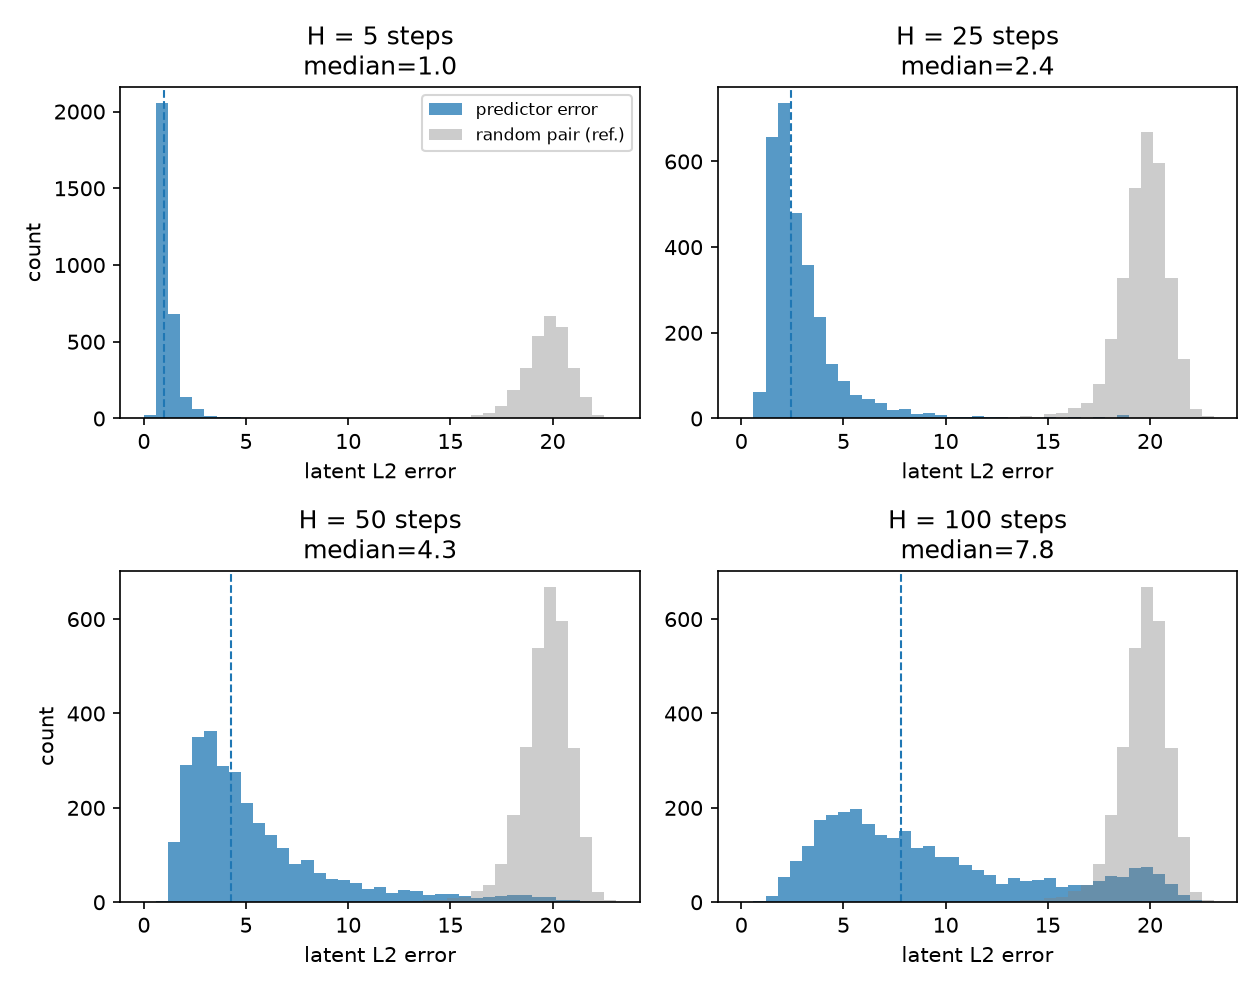
\includegraphics[width=.9\linewidth]{fig_predictor_error_by_horizon}
\caption{Push-T latent rollout error under logged actions as a function of horizon,
with the random-pair latent-distance reference. We evaluate predictions under logged
actions; the errors need not match those on CEM's selected actions.}
\label{fig:predictor-error-by-horizon}
\end{figure}
% BEGIN inlined content: research/table-predictor-error-and-task-distance.tex
\begin{table}[h]
\centering\small
\caption{Push-T: predictor latent rollout error vs.\ the true same-episode start$\to$goal
distance at the same horizon (both $n=3{,}000$/horizon, identically sampled), median $\pm$ std in
latent L2. Random-pair reference: mean 19.6 (theory: $\sqrt2\times13.88\approx19.63$,
\cref{app:gaussian-shell}). Relative error is the predictor-error median divided by the
start$\to$goal-distance median.}
\label{tab:predictor-error-and-task-distance}
\begin{tabular}{lrrrr}
\toprule
& $H=5$ & $25$ & $50$ & $100$ \\
\midrule
predictor error         & $1.00\pm0.56$ & $2.41\pm2.09$ & $4.28\pm3.82$ & $7.80\pm5.35$ \\
start$\to$goal distance & $5.29\pm2.76$ & $17.06\pm4.19$ & $19.45\pm3.29$ & $19.60\pm2.43$ \\
relative error (\%)     & 18.9 & 14.1 & 22.0 & 39.8 \\
\bottomrule
\end{tabular}
\end{table}
% END inlined content: research/table-predictor-error-and-task-distance.tex

\paragraph{Planning and execution length.}
\Cref{tab:replan-frequency-appendix} varies the CEM horizon and executed chunk together.
Five-step plans perform poorly, consistent with a short lookahead missing useful
multi-step approaches. A 100-step commitment also lowers success. The 25-step
configuration performs best in this sweep, which does not cover all possible MPC settings.
\begin{table}[h]
\centering\small
\caption{Push-T L2 success means (\%) for different plan/execution lengths on 50 tasks
and five seeds. Planning horizon equals the executed chunk; the main setting is 25.
The comparison spans 5-, 25-, and 100-step commitments.
Dashes denote settings not evaluated for the corresponding short budget.}
\label{tab:replan-frequency-appendix}
\begin{tabular}{lrrr}
\toprule
Protocol (budget) &5 steps&25 steps&100 steps\\
\midrule
same-episode 25 (50)&64.0&91.2&--\\
same-episode 50 (100)&19.2&40.8&--\\
same-episode 100 (200)&1.2&13.2&5.6\\
cross-episode (250)&4.4&14.4&4.8\\
\bottomrule
\end{tabular}
\end{table}
The 100-step cross-episode setting requires a final budget-limited segment.
The main comparison uses only full 25-step chunks, so that boundary does not arise there.

\subsection{Gaussian-shell diagnostic}
\label{app:gaussian-shell}
An isotropic Gaussian fit to the 2,336,736 Push-T latents uses empirical mean $\mu$
and variance $\sigma^2=\operatorname{tr}(\Sigma)/192$.
Its predicted centered-radius mean and the measured mean are both 13.88.
The covariance participation ratio is
$\operatorname{tr}(\Sigma)^2/\operatorname{tr}(\Sigma^2)=188.5$.
The variance therefore spans many latent directions. This statistic does not establish
a joint Gaussian distribution or independence between same-episode endpoints.
\Cref{fig:gaussian-shell-r-hist} compares the full radius histogram with the fit;
the midpoint comparison appears in the main text (\cref{fig:gaussian-shell-interp}).

\begin{figure}[h]
\centering
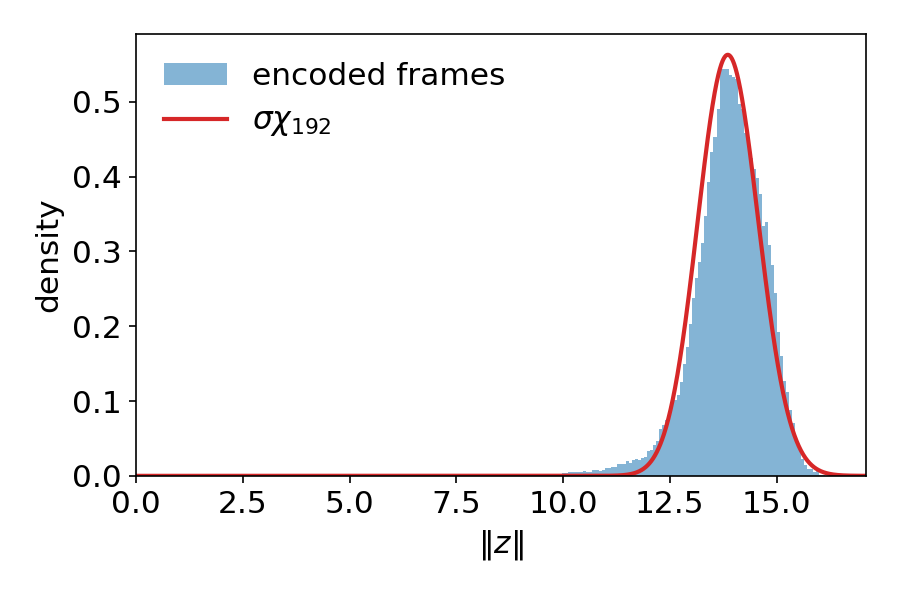
\includegraphics[width=.62\linewidth]{fig_gaussian_shell_r_hist}
\caption{Push-T centered radii of encoded frames and the fitted isotropic Gaussian
reference. Concentrated radii alone do not show that the full latent distribution
is Gaussian or determine which trajectories the action-space planner will choose.}
\label{fig:gaussian-shell-r-hist}
\end{figure}

For 200,000 pairs at offset 100, reported mean endpoint radii are 14.15 and 13.60;
the actual logged midpoint has mean radius 13.81. The arithmetic midpoint has
mean radius 10.03, and 96.4\% of these interpolations lie below the fitted shell's
first-percentile radius.
Straight-line interpolation therefore places most of these midpoints inside the
observed shell, away from the usual data radii. The measurement does not show that
a planner optimizing terminal L2 follows those straight lines.
\Cref{app:separation} explains why shell geometry alone is insufficient to prove a
planning failure.

\subsection{Candidate-ranking diagnostic}
\label{app:cem-trace}
For 25 Push-T tasks per same-episode protocol, the first CEM iteration begins from
the same unadapted population of 300 candidates. The proposed objective selects
30 elites. We execute those candidates in the simulator and compare both costs
with a recovery-time diagnostic that uses simulator state information.
Both costs therefore use the same analyzed candidates, but the proposed objective
selects that subset from the initial population.
% BEGIN inlined content: research/table-cem-trace-rho.tex
\begin{table}[h]
\centering\small
\caption{Mean Spearman correlation between candidate cost and simulator recovery time for the 30 elites selected by the proposed method's first CEM iteration. Of 25 tasks, 25, 24, and 11 have nonconstant diagnostic labels at offsets 25, 50, and 100. We report descriptive correlations without a significance test.}
\label{tab:cem-trace-rho}
\begin{tabular}{lrr}
\toprule
protocol & $\rho$(OUR) & $\rho$(L2) \\
\midrule
same-ep 25  & 0.327  & 0.396 \\
same-ep 50  & 0.203  & 0.086 \\
same-ep 100 & 0.191  & $-$0.064 \\
\bottomrule
\end{tabular}
\end{table}
% END inlined content: research/table-cem-trace-rho.tex
The correlations in \cref{tab:cem-trace-rho} favor L2 at offset 25 and the proposed
score at offsets 50 and 100. Only 11 of 25 offset-100 tasks have nonconstant
recovery labels because of censoring.
We report descriptive correlations on these selected candidates. We do not test
statistical significance or assume that censoring is independent of task difficulty.
The correlations suggest better temporal ranking at longer horizons within this subset.

\section{Compute and reported training settings}
\label{app:params}
\Cref{tab:compute} separates shared encoding, per-seed preparation, and online
decision cost. Summing the listed preparation stages gives 190.8 minutes including
encoding, or 141.2 minutes after shared encoding.
The planning ratio is $1.80/1.14\approx1.58$.
These timings describe one device and can change on other hardware.
\Cref{tab:params} reports component counts. We train both TDR networks and use
only the first during planning.
% BEGIN inlined content: research/table-params.tex
\begin{table}[h]
\centering\small
\caption{Reported component parameter counts on Push-T. We sum the listed components to obtain the frozen subtotal. Rounding accounts for differences between per-member and ensemble totals.}
\label{tab:params}
\begin{tabular}{lr}
\toprule
LeWM encoder (ViT-tiny) & 5.50M \\
LeWM predictor & 10.79M \\
LeWM action encoder & 0.16M \\
\quad Sum of the three listed components & 16.45M \\
\midrule
TDR (used, $\psi_0$ only) & 0.64M \\
TDR (full 2-net ensemble) & 1.29M \\
Critic (per member) & 0.83M \\
Critic (5-member ensemble) & 4.13M \\
\bottomrule
\end{tabular}
\end{table}
% END inlined content: research/table-params.tex

\subsection{Hyperparameters}
\label{app:hyperparams}
\Cref{tab:hyper-shared,tab:hyper-env} list the reported network, optimizer, graph,
and planning settings. The critic maps logits to probability outputs.
We express the integer temporal-efficiency lag $k_{\mathrm{TE}}$ in environment steps
and the graph radius in calibrated TDR units.
The learned components use the shared settings. We set the graph radius and lookahead
from each environment's training-data calibration.
% BEGIN inlined content: research/table-hyper-shared.tex
\begin{table}[h]
\centering\small
\caption{Shared training and planning settings. The critic maps its final scalar logits to probabilities in $[0,1]$. We set the radius and lookahead using each environment's calibration in \cref{tab:hyper-env}.}
\label{tab:hyper-shared}
\begin{tabularx}{\linewidth}{lXr}
\toprule
component & hyperparameter & value \\
\midrule
\multirow{7}{*}{TDR $\psiT$}
 & architecture & 3$\times$512, LN+GELU \\
 & embedding dim & 32 \\
 & expectile $\tau$ & 0.99 \\
 & discount $\gamma$ & 0.99 \\
 & training steps & 50{,}000 \\
 & batch size & 1024 \\
 & learning rate & 3$\times10^{-4}$ \\
\midrule
\multirow{3}{*}{Graph}
 & TE threshold $\theta_{\mathrm{TE}}$ & 0.9 \\
 & clustering radius & $\Htd/2$ \\
 & goal attachment radius & $\max(\Htd,\,1.2\,d_{\min})$ \\
\midrule
\multirow{9}{*}{Critic $V$}
 & ensemble members & 5 \\
 & architecture (per member) & 3$\times$512, SiLU \\
 & max horizon $h_{\max}$ & 50 env steps \\
 & horizon grid & multiples of 5, 0--50 \\
 & training steps & 60{,}000 \\
 & Bellman pessimism $\kappa$ & 1.0 \\
 & loss weights ($\lambda_{\mathrm{Bellman}}$, $\lambda_{\mathrm{mono}}$) & 1.0, 1.0 \\
 & learning rate & 3$\times10^{-4}$ \\
 & EMA target $\tau$ & 0.995 \\
\midrule
\multirow{3}{*}{CEM}
 & population / iterations / elites & 300 / 30 / 30 \\
 & horizon $K$ (blocks $\times$ frameskip) & 5 $\times$ 5 = 25 env steps \\
 & replan interval (receding horizon) & 25 env steps \\
\midrule
\multirow{3}{*}{Criterion (\cref{eq:compose})}
 & critic weight $\beta$ & 1 \\
 & critic cost & $\ET$ from \cref{eq:et} \\
 & final-phase metric & squared latent L2 \\
\bottomrule
\end{tabularx}
\end{table}
% END inlined content: research/table-hyper-shared.tex
% BEGIN inlined content: research/table-hyper-env.tex
\begin{table}[h]
\centering\small
\caption{Environment-specific calibrated TDR scales. $u_k$ is the median distance between training frames $k$ steps apart; $\lambda=u_{25}$ and $r_{\mathrm{TD}}=u_{12}$. The remaining settings listed in \cref{tab:hyper-shared} are shared.}
\label{tab:hyper-env}
\begin{tabular}{lrrr}
\toprule
& Push-T & Reacher & Cube \\
\midrule
$\Htd$ (TDR units) & 7.59 & 3.72 & 7.25 \\
$\lambda=u_{25}$ (TDR units) & 13.53 & 5.83 & 13.63 \\
\bottomrule
\end{tabular}
\end{table}
% END inlined content: research/table-hyper-env.tex

\section{Rendering and action normalization}
\label{app:render}
To check rendering, we render three dataset states again and compare them with
their stored images, requiring mean pixel error within 4/255.
Reacher rendering with MuJoCo 3.12 instead of the dataset's reported 3.5 version
changes the floor texture, with reported average pixel discrepancy 18/255 and
median latent shift 15. The check gives discrepancies of 0.5/255 on Push-T
and at most 0.2/255 on Cube.
This check tests agreement with stored observations; larger changes in renderer
settings could still affect the encoded latents.
Predictor inputs and retrieved action proposals use the full training dataset's
action mean and standard deviation.

\section{Comparison with published evaluations}
\label{app:published}
Panel (B) of \cref{tab:main} reproduces short-horizon results reported by
LeWM \citep{lewm} on its own task sets.
Those results use a different evaluation protocol, so they do not provide paired
comparisons on our fixed tasks.
SAGE reports Push-T success of 64.7\% at offset 150 versus 12.7\% for its LeWM
baseline \citep{sage}. We do not evaluate that offset in the main table.
Our matched comparison establishes improvement over LeWM on the evaluated tasks.
It does not establish superiority over every published planner.
% END inlined content: experiments-appendix.tex
\end{document}
